% Retoca las líneas marcadas con TODO según las necesidades

\documentclass[oneside,a4paper,12pt]{book} % TODO: cambia "oneside" por "twoside" a la hora de imprimirlo

\usepackage[spanish]{babel}
\usepackage[utf8]{inputenc}
\usepackage{geometry}
\usepackage{makeidx}
\usepackage{url}
\usepackage{graphicx}
\usepackage{color}
\usepackage{caption}
\usepackage{acronym}
\usepackage{hyphenat}
\usepackage{a4wide}
\usepackage[normalsize]{subfigure}
\usepackage{float}
\usepackage{titlesec}
\usepackage[Lenny]{fncychap}
\usepackage{listings} % para poder hacer uso de "listings" propios (p.ej. códigos)
\usepackage{eurosym} % para poder usar el símbolo del euro con \euro {xx}
\usepackage{hyperref} % TODO: añade la opción hidelinks para imprimirlo (los enlaces no aparecerán resaltados)

% Para que no parta las palabras
\pretolerance=10000

\newcommand{\bigrule}{\titlerule[0.5mm]} \titleformat{\chapter}[display] % cambiamos el formato de los capítulos
{\bfseries\Huge} % por defecto se usaron caracteres de tamaño huge en negrita
{% contenido de la etiqueta 
\titlerule % línea horizontal 
\filright % texto alineado a la derecha 
\Large\chaptertitlename\ % capítulo e índice en tamaño large
\Large % en lugar de 
\Huge \Large\thechapter} 
{0mm} % espacio mínimo entre etiqueta y cuerpo
{\filright} % texto del cuerpo alineado a la derecha
[\vspace{0.5mm} \bigrule] % después del cuerpo, dejar espacio vertical y trazar línea horizontal gruesa
\geometry{a4paper, left=3.5cm, right=2cm, top=3cm, bottom=2cm, headsep=1.5cm}

% Estilos para ilustrar códigos:
\definecolor{code_green}{rgb}{0,0.6,0}
\definecolor{code_gray}{rgb}{0.5,0.5,0.5}
\definecolor{code_mauve}{rgb}{0.58,0,0.82}

\lstset{frame=tb,
  language=C,
  aboveskip=3mm,
  belowskip=3mm,
  showstringspaces=false,
  columns=flexible,
  basicstyle={\small\ttfamily},
  numbers=none,
  numberstyle=\tiny\color{code_gray},
  keywordstyle=\color{blue},
  commentstyle=\color{code_green},
  stringstyle=\color{code_mauve},
  breaklines=true,
  breakatwhitespace=true,
  tabsize=3
}

\lstset{frame=tb,
  language=C++,
  aboveskip=3mm,
  belowskip=3mm,
  showstringspaces=false,
  columns=flexible,
  basicstyle={\small\ttfamily},
  numbers=none,
  numberstyle=\tiny\color{code_gray},
  keywordstyle=\color{blue},
  commentstyle=\color{code_green},
  stringstyle=\color{code_mauve},
  breaklines=true,
  breakatwhitespace=true,
  tabsize=3
}

\lstset{frame=tb,
  language=Python,
  aboveskip=3mm,
  belowskip=3mm,
  showstringspaces=false,
  columns=flexible,
  basicstyle={\small\ttfamily},
  numbers=none,
  numberstyle=\tiny\color{code_gray},
  keywordstyle=\color{blue},
  commentstyle=\color{code_green},
  stringstyle=\color{code_mauve},
  breaklines=true,
  breakatwhitespace=true,
  tabsize=3
}

% Definición de mis propios tipos: Códigos, Ecuaciones y Tablas
\DeclareCaptionType{code}[Código][Listado de códigos]
\DeclareCaptionType{myequation}[Ecuación][Listado de ecuaciones]

% TODO: especifica las reglas de separación que consideres. Algunos ejemplos:
\hyphenation{fuer-tes}
\hyphenation{mul-ti-ca-pa}
\hyphenation{res-pues-ta}
\hyphenation{di-fe-ren-tes}
\hyphenation{de-sa-rro-lla-dos}
\hyphenation{re-pre-sen-tan-do}

 % archivo de configuración de estilo

\makeindex

\begin{document}
\baselineskip 1.35\baselineskip

\frontmatter

\thispagestyle{empty}
\vspace{2cm}

\begin{figure}[htb]
  \centerline{\resizebox{.60\textwidth}{!}{
\includegraphics{figs/logo_urjc}}}
\end{figure}

\begin{center}
  {\Large {\bf GRADO EN INGENIERÍA DE ROBÓTICA SOFTWARE}}
  \vspace{5mm}
 
  {\large {Escuela de Ingeniería de Fuenlabrada}}
  \vspace{5mm}

  {\large {Curso académico 2022-2023}}

  \vspace{1cm}

  {\large {\bf Trabajo Fin de Grado}}

  \vspace{2cm}

  {\Large {Guide robot navigation\\
               for low-cost robots\\[1cm] }}

  \vspace{5cm}
  {\bf Tutor}: Julio Vega Pérez \\
  {\bf Autor}: Unai Sanz Conejo
\end{center}

\clearpage
\thispagestyle{empty}


% Este diseño se corresponde con la licencia CC-BY-NC-SA.
% Por supuesto, puedes poner la licencia que mejor se adapte al propósito de tu trabajo.
% Recuerda que, si no se especifica ninguna licencia, esta -como cualquier creación artística- pasaría a estar licenciada con todos los derechos reservados (copyright).

\cleardoublepage

\begin{figure}
 \ \ \ \ 
\includegraphics[width=0.25\linewidth]{figs/by-nc-sa.png}
 \label{fig:cc} 
 \end{figure}

\

\

\

\noindent
Este trabajo se distribuye bajo los términos de la licencia internacional \href{http://creativecommons.org/licenses/by-nc-sa/4.0/}{CC BY-NC-SA International License} (Creative Commons AttributionNonCommercial-ShareAlike 4.0). Usted es libre de \textit{(a) compartir}: copiar y redistribuir el material en cualquier medio o formato; y \textit{(b) adaptar}: remezclar, transformar y crear a partir del material. El licenciador no puede revocar estas libertades mientras cumpla con los términos de la licencia:

\begin{itemize}
\item \textit{Atribución}. Usted debe dar crédito de manera adecuada, brindar un enlace a la licencia, e indicar si se han realizado cambios. Puede hacerlo en cualquier forma razonable, pero no de forma tal que sugiera que usted o su uso tienen el apoyo de la licenciante.
\item \textit{No comercial}. Usted no puede hacer uso del material con propósitos comerciales.
\item \textit{Compartir igual}. Si remezcla, transforma o crea a partir del material, debe distribuir su contribución bajo la la misma licencia del original.
\end{itemize}

\begin{flushright}
		\vspace{7.0 cm}
		\emph{Documento de} \textbf{Unai Sanz}. % TODO: pon aquí tu nombre cuando hagas el documento
\end{flushright}



\cleardoublepage

\chapter*{Agradecimientos}

Quisiera expresar mi más sincero agradecimiento a todas las personas que
contribuyeron a la realización de este trabajo. En primer lugar, agradezco al
equipo de ZettaScale por darme la oportunidad de realizar mis prácticas con
ellos y de aprender incontables aspectos acerca de las telecomunicaciones y por
su persistente ayuda. También agradezco a mi tutor de TFG por su orientación
constante y su gran paciencia a lo largo de este proceso.\\

Además estoy profundamente agradecido a mis compañeros de clase por sus ideas y
debates constructivos, que han enriquecido enormemente mi investigación.\\

No puedo dejar de agradecer a mis padres, hermana, amigos cercanos y pareja por
sus ideas, consejos y apoyo moral e incondicional.\\

Por último, pero no menos importante, quiero expresar mi gratitud a todas las
fuentes y recursos que consulté durante la elaboración de este trabajo, así como
a cualquier institución o persona que haya contribuido de alguna manera, aunque
indirecta, a este proyecto.\\

Sin el apoyo de todas estas personas y entidades, este trabajo no habría sido
posible. Gracias de todo corazón.\\

%\ %Separación...

\begin{flushright}
		\vspace{1.5 cm}
		\emph{A mi abuelo;\\
      		  que estaría sumamente orgulloso de mi trabajo.}\\
		\par
		\vspace{1.0 cm}
		Madrid, 31 de Mayo de 2024\\ %\today
		\emph{Unai Sanz}
\end{flushright}

\thispagestyle{empty}



%\begin{verse}
\begin{flushright}
\vspace*{3cm}
\textit{A mi familia\\ 
	(biológica y\\
	 política).}
\end{flushright}
\end{verse}


\cleardoublepage

\chapter*{Resumen\markboth{Resumen}{Resumen}}

%Escribe aquí el resumen del trabajo. Un primer párrafo para dar contexto sobre la temática que rodea al trabajo.\\
%
%Un segundo párrafo concretando el contexto del problema abordado.\\
%
%En el tercer párrafo, comenta cómo has resuelto la problemática descrita en el anterior párrafo.\\
%
%Por último, en este cuarto párrafo, describe cómo han ido los experimentos.


%Primer párrafo (Introducción):
La robótica es un campo amplio que se ha desarrollado con el objetivo de mejorar
la calidad de vida de las personas en numerosos ámbitos.
Existe una gran variedad de robots, cada uno dedicado a un propósito específico,
en el que generalmente igualan o superan el rendimiento humano, incluso
trabajando continuamente sin necesidad de descanso y eliminando riesgos.

%Segundo párrafo (Objetivos):

En este ámbito y con la creciente tendencia a incluir la robótica en el
itinerario formativo, ROS es el software mayormente utilizado, que debido a su
dificultad, resulta difícil de aprender, lo que genera una brecha en la
educación en este campo.
Otro de los grandes problemas de este software reside en su protocolo de
comunicaciones, DDS, el cuál genera una gran cantidad de mensajes, que pueden
saturar la red.
%El presente trabajo por tanto tiene como objetivo dar una solución a estos
%problemas, implementando una forma de programación de flujos de datos compatible
%con ROS2.

%En este ámbito y con la creciente tendencia a incluir la robótica en el
%itinerario formativo, surgen grandes vacíos en cuanto al aprendizaje de este
%campo, siendo ROS el \textit{software} mayormente utilizado en robótica, uno de
%los más complejos y dificiles de aprender para alumnos preuniversitarios.
%Este \textit{software} genera una gran congestión de la red debido al uso de
%DDS como protocolo, reduciendo las posibilidades que ofrece la robótica en el
%aprendizaje, sobre todo en cuanto a la colaboración y coordinación en sistemas
%multirobot, campos cada vez más importantes en un mundo en el que los robots
%son cada vez más comunes.

%Tercer párrafo (Plataforma de desarrollo):
El presente trabajo pretende solucionar estos problemas, utilizando plataformas
\textit{hardware} como los robots Turtlebot 2 y 4, en conjunto con herramientas
\textit{software} como Zenoh-Flow, generando un entorno de programación de
flujos de datos, compatible con nodos existentes de ROS2, haciéndolo más
accesible a los estudiantes de este campo.

%Cuarto párrafo (Arquitectura software con Zenoh y ROS2):
Zenoh-Flow, la herramienta \textit{software} utilizada principalmente, fue
enlazada con ROS2 aprovechando la capacidad del Zenoh-bridge-DDS para
traducir los mensajes entre los protocolos Zenoh y DDS, logrando así una
comunicación bidireccional entre ambos.

%Quinto párrafo (Experimentos):
Los objetivos mencionados fueron alcanzados a través de numerosos experimentos
realizados sobre una aplicación creada siguiendo el paradigma de programación de
flujos de datos con Zenoh-Flow.
En ella, varios robots deben buscar y acercarse a un objeto de manera
organizada, dividiéndose el mapa equitativamente y optimizando trayectorias de
barrido de áreas, de modo que el robot que encuentre dicho objeto, comunique su
posición al resto.

%Sexto párrafo (Conclusiones):
Esto se logró en simulación y, parcialmente debido a errores externos, en un
entorno real de laboratorio, demostrando de esta manera la viabilidad de la
programación de flujos de datos en robótica y su compatibilidad con ROS2.
Asimismo fue demostrada su sencillez, requisito indispensable para su aplicación
en la educación robótica preuniversitaria, ayudando a reducir la brecha
educativa en este ámbito.



\cleardoublepage

\chapter*{Abstract\markboth{Abstract}{Abstract}}



%ENGLISH:
%First paragraph (Introduction):
Robotics is a broad field that has been developed with the aim of improving the
quality of life in numerous areas.
There is a wide variety of robots, each dedicated to a specific purpose,
generally matching or surpassing human performance, even working continuously
without the need for rest and eliminating risks.

%Second paragraph (Objectives):
In the educational field, with the growing trend to include robotics in the
curriculum, ROS is the most widely used software, but due to its difficulty, it
is hard to learn, which creates an educational gap in this field.
Another major problem with this software lies in the use of DDS, a communication
protocol that generates a large number of messages, which can saturate the
network.

%Third paragraph (Development Platform):
This work aims to solve these problems by using hardware platforms such as the
Turtlebot 2 and 4 robots, and software tools like Zenoh-Flow, creating a data
flow programming environment compatible with existing ROS2 nodes, making it more
accessible to students in this field.

%Fourth paragraph (Software Architecture with Zenoh and ROS2):
Zenoh-Flow, the main software tool used, was linked with ROS2 by leveraging
Zenoh-bridge-DDS's capability to translate messages bidirectionally between the
Zenoh and DDS protocols.

%Fifth paragraph (Experiments):
The mentioned objectives were achieved through numerous experiments conducted on
an application created following the data flow programming paradigm with
Zenoh-Flow.
In it, several robots must search for and approach an object in an organized
manner, dividing the map equitably and optimizing area sweeping trajectories, so
that the robot that finds the object communicates its position to the rest.

%Sixth paragraph (Conclusions):
This was achieved in simulation and, partially due to external errors, in a real
laboratory environment, demonstrating the viability of data flow programming in
robotics and its compatibility with ROS2.
Its simplicity was also demonstrated, which is an essential requirement for its
application in pre-university robotics education, helping to reduce the
educational gap in this field.


\cleardoublepage

\chapter*{Acrónimos\markboth{Acrónimos}{Acrónimos}}

% Añade a continuación los acrónimos que uses en el documento. Algunos ejemplos:
\begin{acronym}
	\acro{ROS2}{\emph{Robotic Operating System (ROS) 2}}
	\acro{RMW}{\emph{ROS Middleware Interface}}
	\acro{DDS}{\emph{Data Distribution Service}}
	\acro{STEM}{\emph{Ciencia, Tecnología, Ingeniería y Matemáticas}}
	\acro{NASA}{\emph{National Aeronautics and Space Administration}}
	\acro{JAXA}{\emph{Japan Aerospace Exploration Agency}}
	\acro{UPC}{\emph{Universidad Politécnica de Cataluña}}
	\acro{URJC}{\emph{Universidad Rey Juan Carlos}}
	%\acro{ANN}{\emph{Artificial Neural Network}}
	%\acro{API}{\emph{Application Programming Interface}}
	%\acro{EKF}{\emph{Extended Kalman Filter}}
	%\acro{FOA}{\emph{Focus of Attention}}
	%\acro{GA}{\emph{Genetic Algorithm}}
	%\acro{GPIO}{\emph{General Purpose Input/Output}}
	%\acro{GPS}{\emph{Global Positioning System}}
	%\acro{HCI}{\emph{Human-Computer Interaction}}
	%\acro{HRI}{\emph{Human-Robot Interaction}}
\end{acronym}


\cleardoublepage

\tableofcontents

\listoffigures

\listofcodes

\listofmyequations

\listoftables

%\pagestyle{empty}

\cleardoublepage

 % aquí se cargan todas las "primeras páginas"

% Bibliografía
\let\OLDthebibliography=\thebibliography
\def\thebibliography#1{\OLDthebibliography{#1}
  \addcontentsline{toc}{chapter}{\bibname}}

\mainmatter

\setcounter{page}{1}

\chapter{Introducción}
\label{cap:capitulo1}
\setcounter{page}{1}

\begin{flushright}
\begin{minipage}[]{10cm}
\emph{El éxito es la suma de pequeños esfuerzos repetidos día tras día.}\\
\end{minipage}\\

Robert Collier\\
%Autor, \textit{Título}\\
\end{flushright}

\vspace{1cm}



%[Sección sobre la robótica y la importancia de la exploración espacial]
\section{La evolución y estado de la robótica}
\label{sec:robotica} % etiqueta para luego referenciar esta sección

%[Párrafo sobre la definicion de robótica y de robot]
La robótica es un campo multidisciplinario que se concentra en el diseño,
construcción, programación y operación de robots.
Estos dispositivos electromecánicos, con frecuencia modelados
antropomórficamente o zoomórficamente, están destinados a realizar tareas de
manera autónoma o semiautónoma en una variedad de entornos, para lo que disponen
de sensores que les proveen de información del medio que les rodea, de cierta
capacidad de cómputo para tomar decisiones acerca de estos datos recolectados y
de actuadores que les permiten interactuar con el mismo y llevar a cabo dichas
decisiones, por lo que sus capacidades y limitaciones están detrminadas por su
\textit{hardware}, y su inteligencia reside en su \textit{software}.

%[Párrafo sobre la evolución de la robótica y su aplicación en nuestra sociedad]
Este gran campo de estudio e investigación ha experimentado un rápido
crecimiento y expansión desde sus inicios en la década de 1950, abarcando una
amplia gama de aplicaciones en la industria, la medicina, el entretenimiento y
la exploración espacial, entre muchas otras, y se encuentra en constante
evolución, desempeñando un papel cada vez más importante en nuestra sociedad
moderna, gracias en gran medida a los incesantes avances en tecnologías como la
inteligencia artificial, los sensores, los procesadores y los actuadores.

%[TODO] ¿Añadir imagen de robótica en general en esta sección 1?



%[Sección sobre la importancia de la robótica en los avances científicos]
\section{La importancia de la robótica en los avances científicos}
\label{sec:exploracion_espacial} % etiqueta para luego referenciar esta sección

%[Párrafo sobre la importancia de la propia exploración espacial]
En particular, la robótica ha conformado un factor crucial en la exploración
espacial, y esta ha impulsado la creación de nuevas tecnologías que han sido
desarrolladas exclusivamente para ciertas misiones espaciales pero que luego se
han aplicado en la Tierra, mejorando la calidad de vida de las personas.
Ejemplos destacados incluyen los sistemas de purificación de agua, los tejidos
avanzados como la viscoelástica, los pañales y los dispositivos de imágenes
médicas como la resonancia magnética, que han proporcionado acceso a las
personas respectivamente a agua potable en regiones remotas, a colchones y
almohadas que promueven un mejor descanso, a mayores facilidades en cuanto al
cuidado de los niños y mayores y a diagnósticos médicos precisos sin radiación
nociva, lo cual ha salvado inumerables vidas.
De esta manera, la investigación espacial no solo expande nuestro conocimiento
del universo, sino que también beneficia directamente a la humanidad en la
Tierra.

%[Párrafo sobre el rover Perseverance y el helicóptero Ingenuity]
En cuanto al papel de la robótica en este campo, podemos destacar ejemplos como
los resistentes robots enviados a diferentes planetas y lunas del sistema solar
en busca de datos científicos.
Numerosas misiones científicas lo evidencian, como la misión \textit{Mars 2020}
de la NASA, cuyos robots se ven ilustrados en la Figura \ref{fig:rover}, tomada
por uno de los robots, el rover Perseverance, que depositó con éxito al segundo
robot sobre la superficie marciana, el helicóptero Ingenuity, que aparece más al
fondo en la imagen, y que ayudó al rover a llevar a cabo su exploración y toma
de muestras.
Este helicóptero estaba diseñado para realizar 5 vuelos durante un mes a modo de
demostrador tecnológico, pero su misión pudo alargarse hasta casi los 3 años,
momento en el que termina debido a la rotura de una de sus palas, sumando
entonces un total de 72 vuelos.

\begin{figure} [h!]
  \begin{center}
    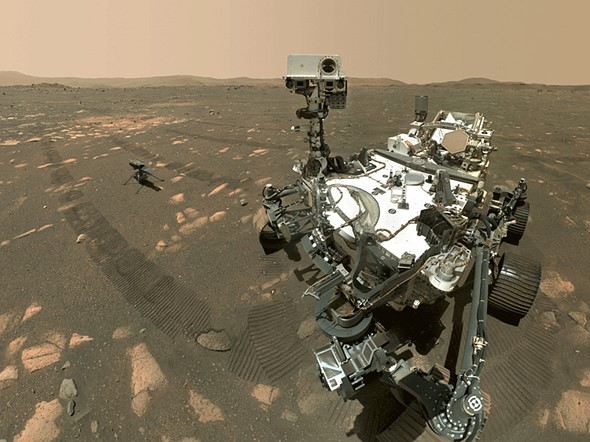
\includegraphics[width=8cm]{figs/perseverance_and_ingenuity_mars_rover_selfie}
  \end{center}
  \caption{Rover Perseverance y helicóptero Ingenuity de la NASA en Marte.}
  \label{fig:rover}
\end{figure}\

%[Párrafo de enlace con la robótica móvil]
Para el éxito de esta misión fue clave la investigación en múltiples campos de
la robótica, como la robótica móvil y todos los campos que esta conlleva, como
pueden ser la visión artificial, la navegación o la localización, áreas clave
que no solo están redefiniendo los límites de la tecnología, sino que también
tienen un gran impacto en cómo usamos la tecnología en nuestra vida diaria, como
ha sucedido por ejemplo, con las aspiradoras robóticas o la conducción
autonoma, que inevitablemente ya forman parte de nuestra sociedad.



%[Sección sobre la robótica móvil y su relación con la educación]
\section{La robótica móvil y su relación con la educación}
\label{sec:robotica_movil} % etiqueta para luego referenciar esta sección

%[Párrafo sobre la robótica móvil]
La robótica móvil ha emergido como un campo multidisciplinario que fusiona la
ingeniería, la inteligencia artificial y múltiples ramas de la robótica y la
mecatrónica para crear sistemas capaces de moverse y operar en entornos
dinámicos, aprovechando áreas como la robótica de campo, la creación de mapas,
la localización y la navegación con ayuda de otros como la visión artificial o
la manipulación de objetos.

Desde sus inicios, ha sido impulsada por los avances tecnológicos, permitiendo
su aplicación en una amplia gama de campos, desde la exploración espacial y
submarina, hasta la logística industrial y la atención médica, siendo ya parte
indispensable de nuestras vidas y mejorando la calidad de las mismas.
En este contexto, la investigación en robótica móvil se centra en desarrollar
sistemas autónomos capaces de navegar de manera segura y eficiente en entornos
conocidos o desconocidos, adaptarse a cambios imprevistos y realizar tareas
complejas de manera autónoma.

Un ejemplo representativo de este tipo de robots se puede ver en la Figura
\ref{fig:boston_dynamics}, donde se pueden observar dos de los robots más
desarrollados en el ámbito móvil, que han demostrado una gran versatilidad en
una variedad de entornos para ejecuatr una amplia variedad de tareas, desde
abrir puertas, pasando por transportar cargas de peso o realizar trabajos
manuales, hasta incluso seguir rutinas de deportivas variadas, que en muchos
casos iguala o incluso supera la de los humanos.

\begin{figure} [h!]
  \begin{center}
    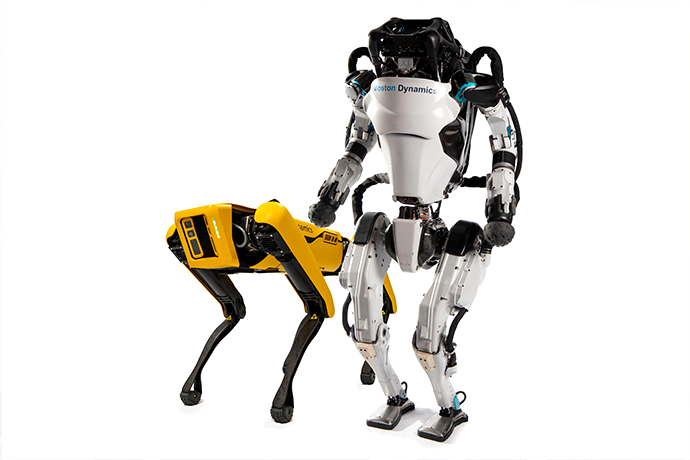
\includegraphics[width=8cm]{figs/atlas_spot_boston_dynamics}
  \end{center}
  \caption{Robots Spot (izq.) y Atlas (dcha.) de Boston Dynamics.}
  \label{fig:boston_dynamics}
\end{figure}\

%[Párrafo introductorio a la localización]
En concreto, la localización de los robots juega una papel importante en la
robótica móvil debido a su indispensable necesidad a la hora de navegar por el
entorno normalmente tomando puntos de referencia gracias a los sensores y
creando un modelo probabilístico de la posición del robot basado en estos datos.

%[Párrafo introductorio a la navegación]
Por su parte, para el correcto funcionamiento de la navegación, es indispensable
conocer la posición del robot durante el movimiento del mismo, para tener la
capacidad de sortear obstáculos y poder desplazar el robot al objetivo.

%\cite{Trawny2009} %multilocalización probabilistica cooperativa unidimensional,
%                  %filtro kalman.
%\cite{Fox2000}    %multilocalización probabilistica basada en sensores y
%                  %balizas visuales.
%[Párrafo introductorio a la multirobótica y trabajos de localización]
La robótica móvil también forma parte de campos más grandes y complejos e
incluso sienta las bases de algunos de ellos, como sucede con la multirobótica,
que representa un paso adelante en la complejidad y la escala de los sistemas
robóticos individuales, y permite realizar tareas que un solo robot no es capaz
de hacer, o realizarlas mucho mas rápidamente o eficientemente.
Como ejemplo de esta ventaja, son notables ciertos trabajos realizados sobre
localización con múltiples robots, como en el artículo \cite{Trawny2009}, en el
que se ponen a prueba las mismas técnicas utilizadas para un solo robot y
evalúan su viabilidad en un entorno unidimensional.
También se han realizado trabajos enfocados a entornos tridimensionales, como se
observa en el artíulo \cite{Fox2000}, en el cuál se logra una localización
basada en sensores, teniendo en cuenta la posición de los demás robots y
aumentando de este modo la precisión de la localización del propio robot en
cuestión.

%[Párrafo sobre la educación en relación con la robótica móvil]
Además, este campo supone una gran oportunidad para el aprendizaje, ya que juega
un papel crucial en el desarrollo de habilidades tecnológicas a la vez que en la
motivación de los estudiantes, los cuales obtienen una gran sensación de
realización y entusiasmo por aprender, al poder viualizar los resultados en
movimiento de manera autonoma.



%[Sección sobre la educación en robótica]
\section{La educación en robótica}
\label{sec:educacion_robotica} % etiqueta para luego referenciar esta sección

%[Párrafo sobre la demanda de educación en robótica en el mundo]
Debido a la creciente participación de los robots móviles en nuestras vidas
diarias, como se ha hecho notar en el caso de las aspiradoras robóticas, la
relevancia de la robótica en el ámbito educativo ha ido ganando terreno en los
últimos años, tanto en la comunidad europea como en otros muchos países.
Esto ha dado lugar a un aumento en la implementación de programas educativos que
han incluido actividades prácticas de robótica en escuelas de educación primaria
y secundaria, promoviendo la creatividad, el pensamiento crítico y las
habilidades tecnológicas entre los estudiantes, además de fomentar el trabajo en
equipo y la resolución de problemas complejos, preparándolos para futuros grados
o carreras relacionadas con la tecnología, cuya demandada aumenta
incesablemente.

%[Párrafo sobre la educación en robótica en España]
En el caso de España, desde la década de los 90, se han implementado programas
piloto y competiciones robóticas, como el programa
Robolot\footnote{https://www.robolot.online/} (1992), desarrollado por la UPC,
las Olimpiadas de Informática \footnote{https://olimpiada-informatica.org/}
(1993), que incorporaron desafíos relacionados con la programación de robots,
así como la RoboCupJunior\footnote{https://junior.robocup.org/} (2000),
ofreciendo a los estudiantes la oportunidad de diseñar, construir y programar
robots para competir en diferentes categorías.
Desde alrededor de 2014, dependiendo de la comunidad autónoma de España, se han
introducido programas y asignaturas que incluyen la robótica como parte esencial
del plan de estudios.

%[Párrafo sobre las herramientas utilizadas en la educación en róbotica]
Al ser necesario un contexto simple y barato para la introducción a la robótica,
en la educación se buscan herramientas como las placas Arduino (Figura
\ref{fig:arduino}), que presentan una amplia compatibilidad con distintos
sensores y actuadores y brinda un entorno sencillo para aquellos que se están
introduciendo en este campo y plataformas como \textit{Scratch}
\footnote{https://scratch.mit.edu/} para simplificar
la programación gracias a su interfaz de bloques y la asociación de ideas a
colores, como se muestra en la Figura \ref{fig:scratch}.

\begin{figure}[h!]
  \centering
  \begin{minipage}{0.45\textwidth}
    \centering
    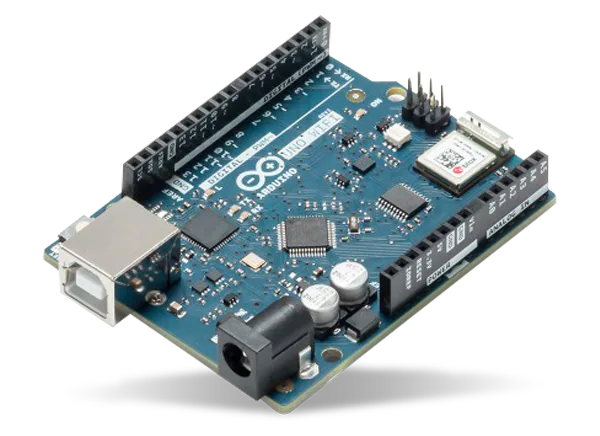
\includegraphics[width=7cm]{figs/arduino}
    \caption{Arduino.}
    \label{fig:arduino}
  \end{minipage}
  \hfill
  \begin{minipage}{0.45\textwidth}
    \centering
    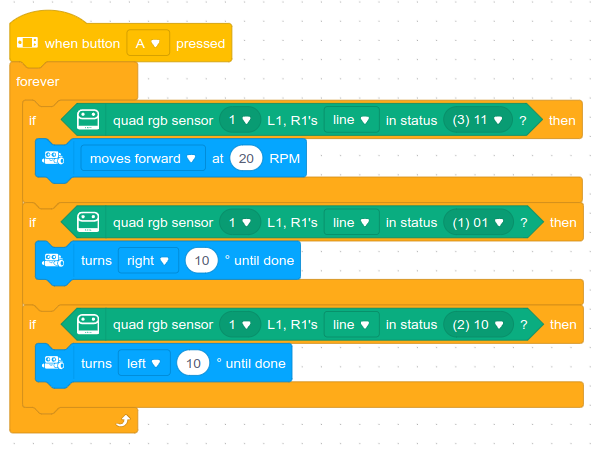
\includegraphics[width=7cm]{figs/scratch_arduino_code}
    \caption{Código de Arduino en Scratch.}
    \label{fig:scratch}
  \end{minipage}
\end{figure}\

%[Párrafo sobre la educación en relacion con la robótica móvil]
Las placas utilizadas en el ámbito educativo, mencionadas anteriormente,
resultan ideales para estos propósitos debido a su coste y simplicidad, sin
embargo, también imponen ciertas limitaciones en las capacidades del robot y en
la posibilidad de añadir \textit{hardware} externo más complejo y potente, como
cámaras o LIDARs, o actuadores como motores más potentes que a menudo requieren
de mayor alimentación eléctrica de la que estas placas pueden brindar.
Esto genera trabas a la propia originalidad y aprendizaje de los estudiantes,
restringiendo así su creatividad, innovación y potencial de creación, una vez se
han obtenido unos conocimientos básicos.

%[Párrafo sobre el escalón de aprendizaje en la educación en robótica]
Es entonces cuando se encuentra el desafío de dar el siguiente paso: la
programación de robots utilizando ROS, el \textit{middleware} estándar por
excelencia en robótica.
Este proceso implica un considerable escalón de aprendizaje, ya que no solo se
debe dominar un lenguaje de programación más complejo, sino que también se debe
comprender el entorno que rodea a esta plataforma, en el que se incluyen campos
de la robótica como son las comunicaciones, la arquitectura \textit{software},
la programación modular y orientada a objetos, algoritmos y estructuras de
datos, entre otros muchos, y que suelen conllevar decenas de asignaturas con
identidad propia en cualquier grado de universidad.
La teoría de la existencia de una brecha educativa en este ámbito se ve
respaldada por trabajos como la tesis doctoral de \cite{vega18b}, en cuyas
secciones A.3 y A.4, se analiza esta misma perspectiva y se propone una solución
respectivamente.

Dicha complejidad puede verse ilustrada en la Figura \ref{fig:ros}, en la que se
muestra un esquema simplificado de la arquitectura de ambas versiones de este
\textit{middleware} que puede resultar abrumadora para aquellos que se están
iniciando en este ámbito, ya que se muestra la creciente complejidad adquirida
al pasar de ROS, que ya era suficientemente complejo, a ROS2, en el que ahora
existen distintas implementaciones de \textit{middleware} de comunicaciones, y
otras capas como al de transporte, el sistema operativo y el \textit{hardware}.

\begin{figure} [h!]
  \begin{center}
    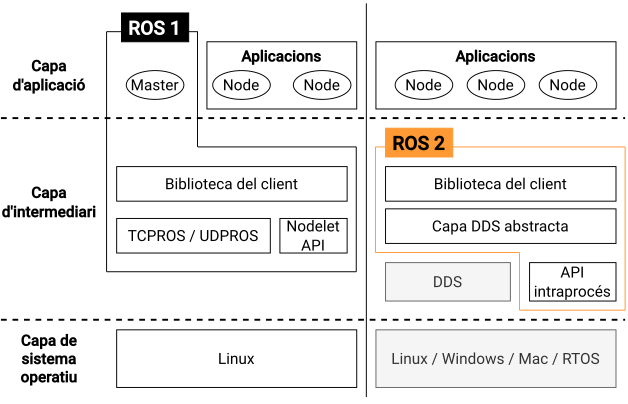
\includegraphics[width=12cm]{figs/ROS_and_ROS2}
  \end{center}
  \caption{Arquitectura de ROS y ROS2.}
  \label{fig:ros}
\end{figure}\

%[Párrafo sobre la solución al escalón de aprendizaje en robótica]
Por este motivo, resulta evidente la necesidad de un paso intermedio que pueda
actuar como puente entre estos dos niveles de aprendizaje, el cual podría ser
incorporado, por ejemplo, en el programa educativo del bachillerato tecnológico
o de centros de educación secundaria.
Este nivel intermedio facilitaría la transición entre las habilidades adquiridas
en la enseñanza primaria o secundaria y los requisitos más avanzados de la
universidad en el campo de la robótica.



%[Sección sobre la robótica de bajo coste]
\section{La robótica de bajo coste}
\label{sec:robotica_bajo_coste} % etiqueta para luego referenciar esta sección

%[Párrafo sobre la robótica de bajo coste]
La robótica de bajo coste se refiere al desarrollo e implementación de sistemas
robóticos como los descritos anteriormente utilizando componentes y recursos
económicos, con el objetivo de hacer la tecnología robótica más accesible y
asequible para una amplia gama de aplicaciones y usuarios.
Este enfoque busca reducir los costes asociados con la construcción y operación
de robots, empleando materiales económicos, hardware de bajo coste y técnicas
de fabricación eficientes.

%[Párrafo sobre la robótica de bajo coste en relación con la robótica móvil]
En el contexto de la robótica móvil, los sistemas de bajo coste pueden ofrecer
soluciones viables para aplicaciones con presupuestos limitados o despliegues a
gran escala, abarcando un papel crucial en áreas como la educación, la
investigación académica, la asistencia social y la exploración de entornos
remotos o peligrosos.
Además de su utilidad práctica, la robótica de bajo coste también promueve la
innovación y el desarrollo de nuevas tecnologías al proporcionar una plataforma
accesible para la experimentación y la creatividad abierta a una amplia
comunidad, así como a la educación.

%[Párrafo ejemplificativo sobre la robótica de bajo coste]
Un ejemplo destacado de este tipo de robótica es el robot Sora-Q representado en
la Figura \ref{fig:sora_q}, enviado a la Luna recientemente por la JAXA y
desarrollado por una empresa de juguetería japonesa, y que tras completar su
misión, fue comercializado por 150\euro, hito que ilustra cómo la tecnología
robótica puede volverse accesible para un público más amplio, incluso
después de su participación en misiones espaciales.

\begin{figure} [h!]
  \begin{center}
    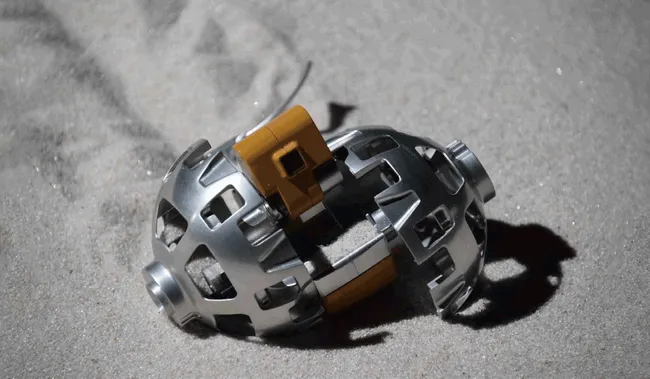
\includegraphics[width=8cm]{figs/SoraQ_lunar_robot_JAXA}
  \end{center}
  \caption{Sora-Q, robot lunar \textit{low-cost} desarrollado por Takara Tomy y la JAXA.}
  \label{fig:sora_q}
\end{figure}\

%[Párrafo sobre la robótica de bajo coste en relación con la educación]
La educación en robótica suele basarse en este tipo de sistemas de bajo coste,
ya que las instituciones educativas enfrentan limitaciones presupuestarias que
dificultan la adquisición de sistemas más costosos, por su gran número de
alumnos, a los que no podrían proveer de sistemas de este calibre de otra
manera.

%[Párrafo sobre los beneficios de la robótica de bajo coste en la educación]
La robótica de bajo coste no solo ha democratizado el acceso a la tecnología
robótica, sino que también ha revolucionado la forma en que se enseña la
robótica en las escuelas.
Este enfoque económico ha permitido a las instituciones educativas superar las
limitaciones presupuestarias y proporcionar a un mayor número de estudiantes la
oportunidad de involucrarse en actividades prácticas de robótica, allanando el
camino para que los estudiantes se sumerjan en áreas más avanzadas de este área,
como pueden ser la robótica móvil o campos estrechamente relacionados.



%[Sección sobre la multirobótica]
\section{La multirobótica}
\label{sec:multirobotica} % etiqueta para luego referenciar esta sección

%\cite{Verma2021}      %Resumen de multirobotica en general.
%\cite{Parker2003}     %Subcampos de multirobotica explicados (comunicación, la
%                      %planificación de tareas, la localización, la creación de
%                      %mapas, la manipulación de objetos, la coordinación de
%                      %robots, o robótica reconfigurable...).
%\cite{Sheng2006}      %Enfocado a descentralizacion, coordinacion y
%                      %optimizacion.
%\cite{Alami1998}      %Cooperacion, menor centralizacion, programar cada robot.
%\cite{Chaimowicz2001} %Coordinacion centralizada, los robots tienen la
%                      %capacidad de cambiar de rol.

%[Párrafo introductorio sobre la multirobótica]
La multirobótica es un campo de investigación que estudia y desarrolla sistemas
robóticos compuestos por múltiples robots que trabajan en conjunto para realizar
una variedad tareas complejas, que ha sido ampliamente estudiada en artículos
como \cite{Verma2021}, en los que se relatan todos los aspectos de la misma,
poniendo en contexto este novedoso campo.

%[Párrafo más específico sobre las tareas más relevantes en la multirobótica]
Estos sistemas pueden dividir sus tareas, como la exploración de entornos
desconocidos o la búsqueda y rescate en áreas de difícil acceso, por lo que la
colaboración entre ellos es de vital importancia, e implica aspectos como el
establecimiento de comunicaciones para compartirse información y entender de un
mejor modo el mundo y contexto que les rodea, la creación de mapas del entorno
para poder localizarse y navegar por el mismo de manera controlada o la
manipulación de objetos, muchas veces necesaria para completar el objetivo
propuesto para estos sistemas.
Todo ello puede verse descrito en al trabajo de \cite{Parker2003}, en el que se
relatan con más detalle los avances logrados en estos aspectos.

%[Párrafo sobre la importancia de la coordinación en la multirobótica]
La coordinación entre estos sistemas puede suponer la diferencia entre el éxito
o el fracaso de su misión, por lo que también es de suma importancia, y por ello
se han realizado múltiples trabajos acerca de este tema.
En estos términos, los equipos de robots pueden operar eficientemente
asignando roles y responsabilidades como expone el artículo de \cite{Alami1998},
en el que se desarrolla un sistema de control con la menor centralización
posible para estudiar la cooperación multirobot en el proyecto MARTHA.

%[Párrafo sobre la descentralización en la multirobótica]
A pesar de intentar crear sistemas con la mayor descentralización posible, el
trabajo anterior sigue siendo un sistema centralizado, donde un robot puede
asumir roles específicos.
La tendencia actual se inclina hacia sistemas directamente o casi totalmente
descentralizados, donde la coordinación y la optimización son fundamentales,
como es notable en el trabajo de \cite{Sheng2006}, en el que todos los robots
actualizan su propio mapa local con la información de los demás, sin que ninguno
de ellos adquiera un mayor protagonismo o importancia.

Gracias a este tipo de trabajos, se ha conseguido mejorar la eficiencia y la
robustez de los sistemas robóticos, y la multirobótica se ha convertido en un
campo importante de investigación.
Los principios y problemas técnicos en este campo se exploran en diversos
contextos, como se ilustra en la Figura \ref{fig:multirobots}, en la cual, la
flota de robots está realizando una tarea de búsqueda y rescate, mediante la
división de un área, probablemente desconocida, actualizando sus mapas como
se ha explicado anteriormente.

\begin{figure} [h!]
  \begin{center}
    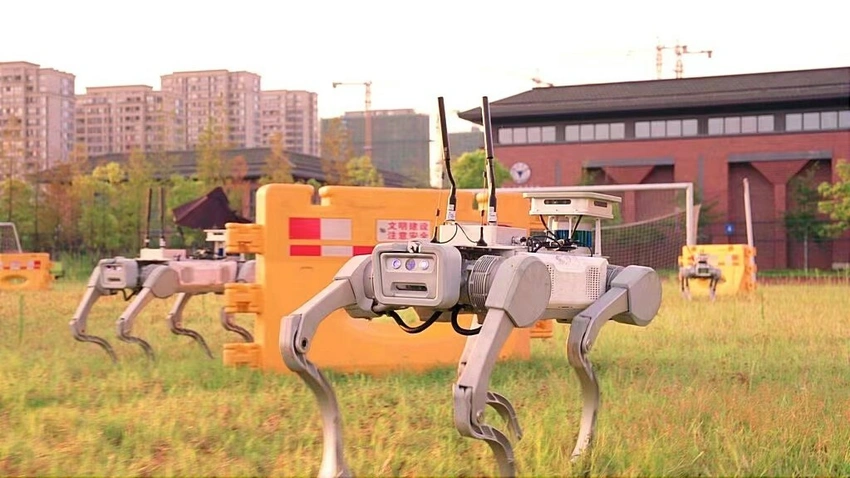
\includegraphics[width=8cm]{figs/multirobotics_in_search_and_rescue}
  \end{center}
  \caption{Múltiples robots durante una operacion de búsqueda y rescate.}
  \label{fig:multirobots}
\end{figure}\

%[Párrafo sobre la multirobótica en educación].
En el ámbito educativo, la multirobótica ofrece una oportunidad única para
involucrar a los estudiantes en actividades prácticas y colaborativas.
Al trabajar con sistemas multirobot, los estudiantes no solo adquieren
conocimientos sobre programación, control y mecánica de robots, sino que también
exploran conceptos como son las telecomunicaciones entre robots, la coordinación,
la planificación y asignación de tareas con o sin prioridades, la localización y
navegación conjunta, como se ha explicado en los trabajos citados en la sección
\ref{sec:robotica_movil}, así como la seguridad que se requiere para evitar
colisiones entre ellos, adquiriendo a su vez habilidades útiles para el trabajo
en equipo.
Además, la multirobótica proporciona un entorno de aprendizaje dinámico y
estimulante que despierta aún más la curiosidad y la creatividad de los
estudiantes, preparándolos para enfrentar los desafíos del mundo tecnológico en
constante evolución.

%[Párrafo sobre ejemplos de múltiples robots educativos].
Un ejemplo representativo de los robots educativos, en este caso del laboratorio
de robótica de la URJC, aparece en la Figura \ref{fig:robots_education}, en la
que se pueden diferenciar hasta dos modelos distintos de robots: Turtlebot 2 en
la parte superior de la imagen, y Turtlebot 4, más modernos, en la parte inferior
de la misma.

\begin{figure} [h!]
  \begin{center}
    \includegraphics[width=8cm]{figs/multirobotics_education}
  \end{center}
  \caption{Robots educativos, modelos Turtlebot 2 (arriba) y Turtlebot 4 (abajo).}
  \label{fig:robots_education}
\end{figure}\



%[Sección sobre los flujos de datos en robótica]
\section{Flujos de datos en robótica}
\label{sec:flujos_datos} % etiqueta para luego referenciar esta sección

%[Párrafo sobre las telecomunicaciones entre robots]
Las mencionadas telecomunicaciones entre robots son fundamentales en la
multirobótica, ya que garantizan una comunicación rápida, optima, eficiente y
ordenada entre los distintos dispositivos, necesaria para un correcto desempeño
de la funcionalidad en cuestión.
Sin embargo, este proceso puede enfrentarse a desafíos como la congestión de la
red, y la consecuente pérdida de mensajes, que pueden ser críticos para el
correcto funcionamiento de los robots.
Por este motivo es crucial gestionar cuidadosamente la cantidad de robots y
mensajes generados, intentando minimizarlos para optimizar el rendimiento del
sistema y evitando de esta manera el problema conocido como \textquotedblleft
cuello de botella\textquotedblright.

%[Párrafo sobre las ZettaScale]
Una de las empresas más importantes en este ámbito es ZettaScale Technology, que
ha tomado mucha relevancia en los últimos años, ya que es responsable de una de
las implementaciones de \textit{middleware} de telecomunicaciones de DDS
utilizado en ROS2, llamado \textit{CycloneDDS} y son los desarrolladores de un
nuevo protocolo de comunicaciones llamado \textit{Zenoh}, que ya cuenta con
importantes clientes como la NASA, debido a las prestaciones que este ofrece,
superando en la mayoria de casos a los protocolos convecionales y que ya ha sido
oficialmente seleccionado como el próximo RMW de ROS2
\footnote{https://discourse.ros.org/t/ros-2-alternative-middleware-report/33771}.
Además de esto poseen un potente middleware para la programación de flujos de
datos aún en desarrollo, llamado \textit{Zenoh-Flow}, así como un puente llamado
\textit{zenoh-bridge-dds} que hace las veces de traductor entre los protocolos
DDS y Zenoh, lo que permite la comunicación entre estos flujos de datos con
nodos de ROS2, haciendo posible la creación de aplicaciones robóticas en forma
de flujos de datos, utilizando nodos de ROS2 existentes, y fusionando de esta
manera ambos campos.

%[Párrafo sobre flujos de datos y comportamiento reactivo mas simple para educación]
Mantener un flujo de datos correcto es fundamental para solventar los problemas
de telecomunicaciones mencionados en el desarrollo de sistemas de multirobótica.
Además, simplifica el desarrollo del software al proporcionar una clara visión
de la dirección, el origen y el destino de los datos en cada momento.
Esto permite dividir el programa en partes claramente diferenciadas, normalmente
llamadas nodos, modularizándolo y dando lugar a la división del problema último
en varios problemas más simples y fáciles de atajar.
Como resultado, el desarrollo se vuelve un proceso más sostenible y escalable, y
por tanto, más fácil de llevar a cabo por los estudiantes.

Podemos ver ejemplificado este proceso en la Figura \ref{fig:data_flow}, donde
se ilustra el flujo de datos de manera simplificada, de un robot para detectar y
seguir códigos QR\footnote{https://github.com/USanz/follow_beacon}, en la que se
puede observar cómo lo los datos siguen un esquema de nodos dirigido, y en este
caso unidireccional, pasando de su orígen en el robot a su procesamiento en otra
máquina y acabando en su posterior vuelta al robot en forma de ordenes de
movimiento, pudiendo saber en todo momento en qué proceso se encuentran dichos
datos.

\begin{figure} [h!]
  \begin{center}
    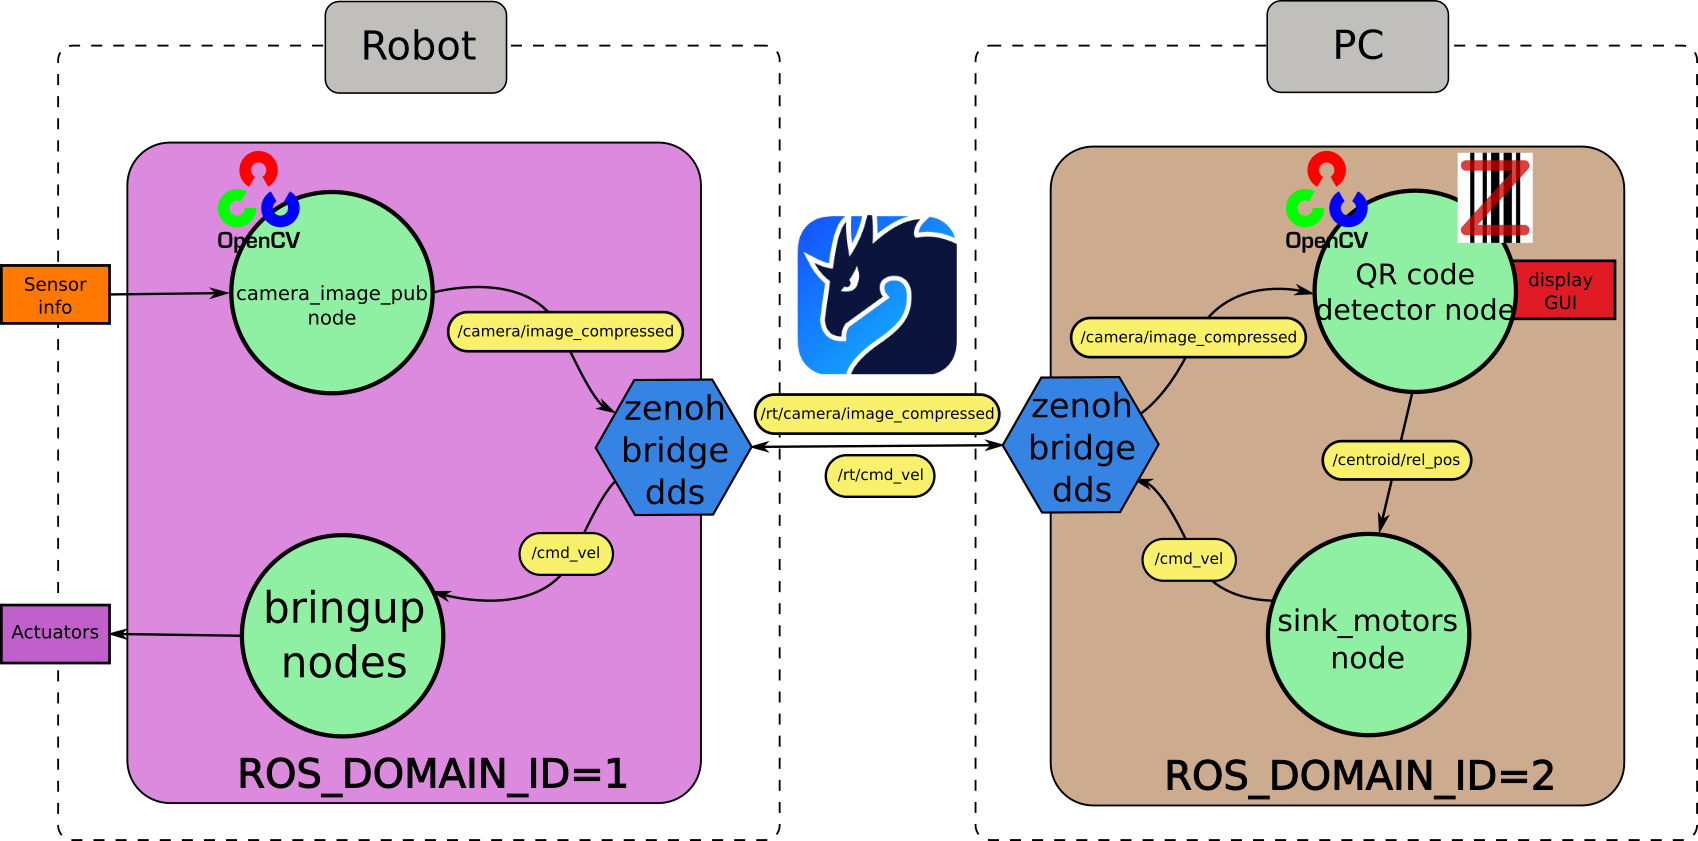
\includegraphics[width=15cm]{figs/QR_code_data_flow}
  \end{center}
  \caption{Flujo de datos de un robot para la detección y seguimiento de códigos QR.}
  \label{fig:data_flow}
\end{figure}\

%[TODO] ¿citar mi propio trabajo follow_beacon? No.
%[TODO] Que lo entienda mi madre.
%[TODO] Eliminar comentarios sobrantes al final (moverlos a su sección).
%[TODO] Capitulo II Estado del arte (no necesario si cito bien todo en la introduccion).
%[TODO] Hacer collage de las imagenes del video para explicar en varios pasos lo mismo que el video.
%[TODO] Poner las URLs como notas al pie. Ej: Robocup\footnote{\url{http://www.robocup.org}}.
%[TODO] Poner las URLs de videos en las notas al pie de página??











%[TODO] Párrafo de la antigua introducción que debería ser movido posiblemente
% al siguiente capitulo (hay cosas repetidas):

%La educación en robótica se basa en la robótica de bajo coste, normalmente en
%placas como Arduino o similares, las cuales son ideales para este uso, y a su
%vez limitan la capacidad del robot en cuestión y el hardware que se puede usar y
%consecuentemente limitan la creatividad y el aprendizaje de los niños. Una vez
%se llega a un cierto nivel de conocimientos, el siguiente paso suele ser la
%programación de robots con ROS2, donde existe un gran escalon de aprendizaje.
%Este trabajo busca simplificar el desarrollo del software en ROS2 y así reducir
%dicho escalón, para hacer más fácil este desarrollo, dando la posibilidad de
%crear aplicaciones robóticas más complejas para robots más completos y que
%permanecen dentro de la categoría de robots de bajo coste y por tanto siguen
%siendo asequibles para instituciones como colegios o institutos.\\

%Escribe aquí un párrafo explicando brevemente lo que vas a contar en este capítulo. En este primer capítulo, el de introducción, se trata de dar un contexto amplio y atractivo del trabajo. Comienza hablando de un contexto general y acaba hablando del contexto más específico en el que se enmarca el proyecto. Es el capítulo idóneo para incluir todas las referencias bibliográficas que hayan tratado este tema; suponen un fuerte respaldo al trabajo.\\

%\section{Problemas de ROS en relación con el aprendizaje}
%\label{sec:miseccion} % etiqueta para luego referenciar esta sección

%\section{Problemas de ROS en relación con el aprendizaje}
%\label{sec:miseccion} % etiqueta para luego referenciar esta sección

%ROS es el estándar en robótica para la programación de robots, pero tiene un
%problema y es el gran escalón de aprendizaje que existe cuando se pasa de una
%placa simple como arduino, a robots más complejos con máquinas integradas como
%las placas Raspberry Pi o un ordenador portátil directamente. Esto conlleva a una gran
%diferencia entre la robótica que se enseña en los colegios e institutos a la que
%se ebnseña en universidades, y es debido precisamente a la complejidad de código
%y enseñanza de ROS, para los cuales, se requiere incluso de varias asignaturas.
%Por eso en este trabajo se pretende incorporar un paso intermedio en este gran
%escalón.
%
%La propia naturaleza de este \textit{middleware} robótico nos obliga a programar
%nodos que se ejecutan iterativamente en bucle, sin necesidad de generar una
%topología de red concreta para saber de donde vienen o a donde van los datos, lo
%que puede ser un poco complicado de entender a primera vista para los niños.\\
%
%Además de este problema, existe otro relacionado con la congestión de red: los
%nodos de ROS2 se comunican a través de DDS, un protocolo de comunicaciones que
%genera una gran cantidad de mensajes de \textit{Discovery}, lo que conlleva
%consecuentemente a la generación de congestión de la red, y dificulta de esta
%manera la programacion de aplicaciones multirobóticas, que son un posible
%siguiente paso en la enseñanza de la robotica, para entender las comunicaciones
%entre los distintos robots.\\
%
%Este trabajo prentende solucionar tanto el problema del escalón de aprendizaje,
%suponiendo un paso intermedio en la enseñanza de la robótica, y el problema de
%la congestión de red generala por DDS, suponiendo una posible solución a la
%misma.\\
%
%El problema de la congestión se soluciona usando otro protocolo llamado Zenoh,
%con mejores prestaciones que DDS, y la simplicidad del código de ROS2, se ha
%conseguido gracias al uso de un \textit{framework} llamado Zenoh-Flow, que
%funciona sobre el protocolo mencionado y el cual le da nombre. Este
%\textit{framework} está pensado para la programación de flujos de datos,, por lo
%que hay que definir primero un flujo de datos que luego seguiran los nodos,
%activando su iteración al momento de recibir un dato, generando de esta manera
%un flujo de datos que pasa de nodo a nodo, a diferencia de ROS.\\
%
%La implementación conjunta con ROS es posible gracias a que Zenoh-flow permite
%serializar los datos que se quieren enviar, y existe un bridge que los traduce
%de Zenoh a DDS para que los nodos de ROS2 entiendan dicha información. Es por
%este motivo, que si se serializan los mensajes de la misma manera que se hace
%internamente en ROS2, se pueden seguir utilizando nodos ya implementado en ROS2,
%como puede ser la navegación.\\

%En los textos puedes poner palabras en \textit{cursiva}, para aquellas expresiones
%en sentido \textit{figurado}, palabras como \textit{robota}, que está fuera del
%diccionario castellano, o bien para resaltar palabras de una colección:
%\textit{(a)} es la primera letra del abecedario, \textit{(b)} es la segunda, etc.\\

%Al poner las dos líneas del anterior párrafo, este aparecerá separado del anterior. Si no las pongo, los párrafos aparecerán pegados. Sigue el criterio que consideres más oportuno.

%\section{Segunda sección}
%\label{sec:segundaseccion}
%
%No olvides incluir imágenes y referenciarlas, como la Figura \ref{fig:roomba}.
%
%\begin{figure} [h!]
%  \begin{center}
%    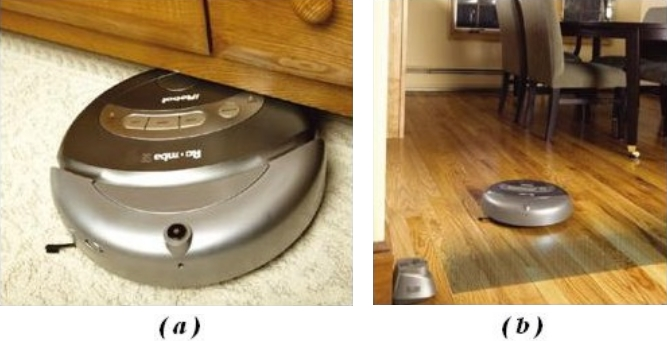
\includegraphics[width=8cm]{figs/roomba}
%  \end{center}
%  \caption{Robot aspirador Roomba de iRobot.}
%  \label{fig:roomba}
%\end{figure}\
%
%Ni tampoco olvides de poner las URLs como notas al pie. Por ejemplo, si hablo de la Robocup\footnote{\url{http://www.robocup.org}}.
%
%\subsection{Números}
%\label{sec:subseccion}
%
%En lugar de tener secciones interminables, como la Sección \ref{sec:miseccion}, divídelas en subsecciones.
%
%Para hablar de números, mételos en el entorno \textit{math} de \LaTeX, por ejemplo, $1.5Kg$. También puedes usar el símbolo del Euro como aquí: 1.500\euro.
%
%\subsection{Listas}
%
%Cuando describas una colección, usa \texttt{itemize} para ítems o \texttt{enumerate} para enumerados. Por ejemplo:
%
%\begin{itemize}
% \item \textit{Entorno de simulación.} Hemos usado dos entornos de simulación: uno en 3D y otro en 2D.
% \item \textit{Entornos reales.} Dentro del campus, hemos realizado experimentos en Biblioteca y en el edificio de Gestión.
%\end{itemize}\
%
%\begin{enumerate}
% \item Primer elemento de la colección.
% \item Segundo elemento de la colección.
%\end{enumerate}\
%
%\paragraph{Referencias bibliográficas}
%\label{sec:referencias}
%
%Cita, sobre todo en este capítulo, referencias bibliográficas que respalden tu argumento. Para citarlas basta con poner la instrucción \verb|\cite| con el identificador de la cita. Por ejemplo: libros como \cite{vega12e}, artículos como \cite{vega19b}, URLs como \cite{vega19a}, tesis como \cite{vega18b}, congresos como \cite{vega18a}, u otros trabajos fin de grado como \cite{vega08b}.
%
%Las referencias, con todo su contenido, están recogidas en el fichero \texttt{bibliografia.bib}. El contenido de estas referencias está en formato \texttt{BibTex}. Este formato se puede obtener en muchas ocasiones directamente, desde plataformas como \texttt{Google Scholar} u otros repositorios de recursos científicos.
%
%Existen numerosos estilos para reflejar una referencia bibliográfica. El estilo establecido por defecto en este documento es APA, que es uno de los estilos más comunes, pero lo puedes modificar en el archivo \texttt{memoria.tex}; concretamente, cambiando el campo \verb|apalike| a otro en la instrucción \verb|\bibliographystyle{apalike}|. 
%
%\
%
%\
%
%\
%
%Y, para terminar este capítulo, resume brevemente qué vas a contar en los siguientes.


\chapter{Objetivos}
\label{cap:capitulo2}

\begin{flushright}
\begin{minipage}[]{10cm}
\emph{Dame seis horas para talar un árbol y pasaré las primeras cuatro afilando el hacha}\\
\end{minipage}\\

Abraham Licoln\\
\end{flushright}

\vspace{1cm}

Una vez establecido el marco contextual de este proyecto, se procederá a
presentar una descripción del problema abordado, así como el proceso creativo e
intelectual que ha guiado el desarrollo del mismo, que incluirá los requisitos
del proyecto, la metodología empleada y el plan de trabajo detallado.

%Escribe aquí un párrafo explicando brevemente lo que vas a contar en este capítulo. En este capítulo lo ideal es explicar cuáles han sido los objetivos que te has fijado conseguir con tu trabajo, qué requisitos ha de respetar el resultado final, y cómo lo has llevado a cabo; esto es, cuál ha sido tu plan de trabajo.\\

\section{Descripción del problema}
\label{sec:descripcion}

Este proyecto surge como respuesta a la escasa investigación sobre los flujos de
datos en conjunto con ROS2, ofreciendo a su vez un entorno propicio para la
creación sencilla de distintas aplicaciones robóticas basadas en dichos flujos
de datos, que pueden replicar de manera versátil y sencilla, los comportamientos
reativos de los robots, eludiendo la complejidad inherente de este
\textit{middleware} robótico y dando lugar, por tanto, a un nuevo entorno de
programación más simple.

Además, tiene como objetivo secundario cerrar la brecha educativa entre la
enseñanza secundaria y universitaria, expuesta en la Sección
\ref{sec:educacion_robotica}, en la que queda explicado el salto que existe en
la educación en robótica entre la educación secundaria y la universitaria,
debido a la complejidad del código y de las plataformas de desarrollo
utilizadas.

%Cuenta aquí el objetivo u objetivos generales y, a continuación, concrétalos mediante objetivos específicos.

\section{Requisitos}
\label{sec:requisitos}

Para solucionar lso problemas descritos, este trabajo debe cumplir los
siguientes requisitos:

\begin{enumerate}
    \item{Se utilizará \textit{GNU/Linux}, con la distribución
        \textit{Ubuntu 22.04 LTS} como sistema operativo en todos los
        \textit{hardwares}.}
    \item{Desarrollar alguna forma de programación de flujos de datos con ROS2.}
    \item{El entorno de programación debe brindar la posibilidad de funcionar en
        conjunto con nodos de ROS2, permitiendo la comunicación con los mismos
        mediante \textit{topics}.}
    \item{Los \textit{softwares} utilizados deben ser compatibles para funcionar
        correctamente en conjunto.}
    \item{Las aplicaciones demostrativas desarrolladas deben ser fácilmente
        reproducibles y desplegables tanto en un entorno simulado como en un
        ambiente educativo real o de laboratorio.}
    \item{El desarrollo del \textit{software} debe ser lo suficientemente
        sencillo para poder ser llevado a cabo por alumnos preuniversitarios.}
    \item{El \textit{hardware} utilizado debe ser suficientemente económico para
        ser adquirido por organismos educativos.}
\end{enumerate}

Las competencias generales que se han cumplido, según la guía docente de la
asignatura consisten en:

\begin{enumerate}
    \item{\textit{CB2.} Que los estudiantes sepan aplicar sus conocimientos a su
        trabajo o vocación de una forma profesional y posean las competencias
        que suelen demostrarse por medio de la elaboración y defensa de
        argumentos y la resolución de problemas dentro de su área de estudio.}
        Esta competencia ha sido cumplida con la realización de la parte del
        software de este trabajo, en la que se han aplicado distintos
        conocimientos adquiridos durante el grado.
    \item{\textit{CB4.} Que los estudiantes puedan transmitir información,
        ideas, problemas y soluciones a un público tanto especializado como no
        especializado.}
        Esta competencia queda resuelta al detallar todo el complejo proceso
        consecuente a este trabajo de manera clara y comprensible en la memoria
        que esta siendo leída.
    \item{\textit{CB5.} Que los estudiantes hayan desarrollado aquellas
        habilidades de aprendizaje necesarias para emprender estudios
        posteriores con un alto grado de autonomía.}
        Esta competencia queda cumplida al haber adquirido los conocimientos
        suficientes para el desarrollo de este trabajo de manera completamente
        autónoma, a base de distintas pruebas y consultas en Internet.
\end{enumerate}

La competencia específica \textit{CE28} de la asignatura detalla lo
siguiente:
Desarrollo de las capacidades adecuadas para realizar un ejercicio original
individual (o excepcionalmente colectivo), presentarlo y defenderlo ante un
tribunal universitario, consistente en un proyecto en el ámbito de las
tecnologías específicas del campo de la Robótica de naturaleza profesional en el
que se sinteticen e integren las competencias adquiridas en las enseñanzas.
Esta última queda cumplida con la creación del presente trabajo, de la
consecuente memoria y documentación y de su posterior defensa ante un tribunal.

%Describe los requisitos que ha de cumplir tu trabajo.

\section{Metodología}
\label{sec:metodologia}

La metodología utilizada sigue pautas de invesigación sobre el estado del arte
previo al trabajo, y posteriormente sobre el \textit{software} utilizado,
siempre evaluando de antemano la compatibilidad con el \textit{hardware}
disponible, así como realizando pruebas pertinentes sobre su correcto
funcionamiento en los distintos entornos, incluyendo la simulación y el
laboratorio.

En relación con el desarrollo del \textit{software} demostrativo se sigió un
ciclo de desarrollo \textit{software} iterativo, que consiste en la
planificación del \textit{software}, el desarrollo del mismo, su consecuente
revisión mediante pruebas y su corrección, todo ello de manera periódica,
generando en cada una de las iteraciones un resultado ejecutable mejor que el
anterior, hasta conseguir al final una versión completamente funcional, como se
ve reflejado en el esquema de la Figura \ref{fig:desarrollo_iterativo}.
Este proceso de desarrollo puede verse alineado con los principios de mejora
continua del ciclo de desarrollo PDCA.

\begin{figure} [h!]
    \begin{center}
      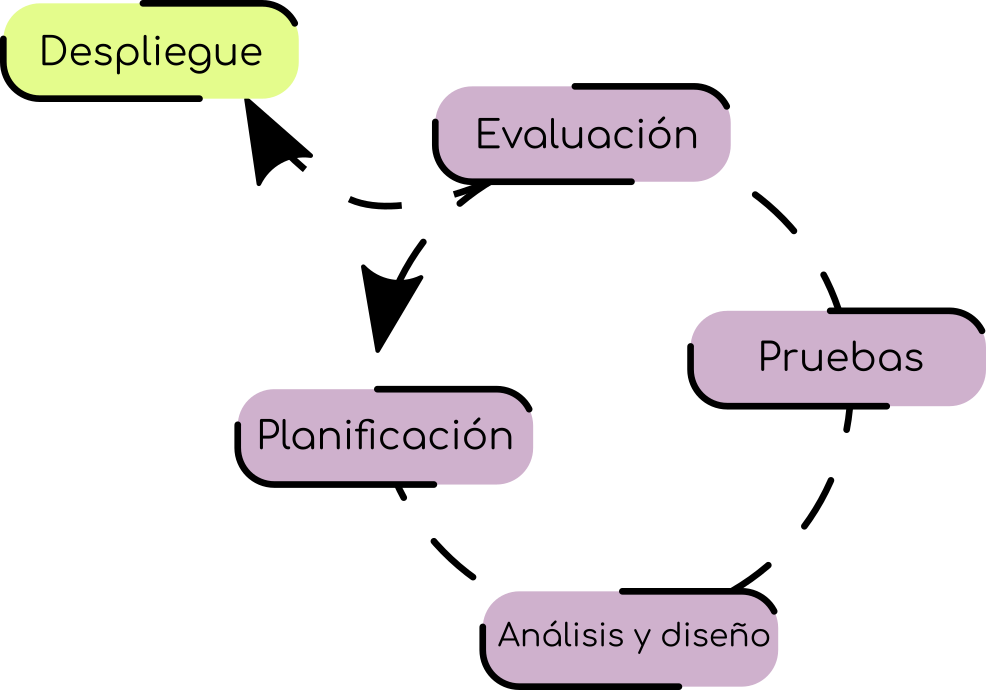
\includegraphics[width=12cm]{figs/desarrollo_iterativo}
    \end{center}
    \caption{Esquema del desarrollo software iterativo.}
    \label{fig:desarrollo_iterativo}
  \end{figure}\

Este desarrollo implicó pruebas periódicas en simulación con el fin de
identificar errores y perfeccionar los valores de los parámetros, para
posteriormente evaluar su funcionamiento en un entorno real, como el del
laboratorio.

%Qué paradigma de desarrollo software has seguido para alcanzar tus objetivos.

\section{Plan de trabajo}
\label{sec:plantrabajo}

El desarrollo del proyecto ha comprendido varias etapas, incluyendo la
investigación del \textit{software} a utilizar, la investigación del estado del
arte, la implementación de una arquitectura \textit{software} funcional en los
distintos entornos y el desarrollo del \textit{software} demostrativo o de
ejemplo, comprendiendo un periodo de tiempo superior a un año, comenzando en
Febrero de 2023 y finalizando en Mayo de 2024.

% [TODO] modificar la fecha final.

\begin{enumerate}
    \item{\textit{Investigación del software a utilizar.} Periodo de febrero a
        mayo de 2023 durante las prácticas de empresa, en las que estuve
        aprendiendo el funcionamiento de \textit{softwares} como Zenoh,
        Zenoh-Flow, Zenoh-bridge-DDS, CycloneDDS, y acerca de las
        telecomunicaciones entre robots, 35 horas semanales durante 4 meses.}
    \item{\textit{Investigación del estado del arte.} Periodo de junio a agosto
        de 2023, en el que se investigó acerca de los trabajos previos
        relacionados, y sobre la viabilidad y compatibilidad del proyecto.}
    \item{\textit{Implementación de una arquitectura software funcional en
        simulación.} Periodo de junio a agosto de 2023, en el que se consiguió
        un corecto funcionamiento del \textit{software} en simulación.}
    \item{\textit{Desarrollo de software demostrativo.} Periodo de agosto a
        noviembre de 2023 en el que se migró el \textit{software} desarrollado
        durante las prácticas a versiones posteriores.}
    \item{\textit{Implementación de una arquitectura software funcional en un
        entorno real.} Periodo de noviembre de 2023 a enero de 2024 en el que se
        consiguió un corecto funcionamiento del \textit{software} en el
        laboratorio.}
    \item{\textit{Pruebas del software desarrollado en el laboratorio.} Periodo
        de noviembre de 2023 a abril de 2024 en el que se realizaron las pruebas
        y cambios necesarios para un corecto funcionamiento del
        \textit{software} demostrativo en el entorno real del labratorio.}
\end{enumerate}

Durante los periodos de desarrollo de este proyecto fuera de las prácticas de
empresa, se dedcaban aproximadamente de 30 a 40 horas semanales entre las que se
incluyen reuniones con el tutor, que generalmente se llevaban a cabo
semanalemente aunque ocasionalmente cada dos semanas.
Este proceso continuo dió lugar a más de un año de esfuerzo.

El proceso de trabajo ha sido realizado mediante contribuciones a un repositorio
en GitHub\footnote{https://github.com/RoboticsURJC/tfg-unai}, así como su
posterior explicación y desarrollo en el apartado de la
Wiki\footnote{https://github.com/RoboticsURJC/tfg-unai/wiki} del mismo, haciendo
las veces de bitácora, donde quedan reflejados todos los contratiempos,
soluciones y pruebas realizados.

%Qué agenda has seguido. Si has ido manteniendo reuniones semanales, cumplimentando objetivos parciales, si has ido afinando poco a poco un producto final completo, etc.


\chapter{Plataforma de desarrollo}
\label{cap:capitulo3}

\begin{flushright}
\begin{minipage}[]{10cm}
\emph{Un buen artesano no se separa nunca de sus herramientas, las conoce y las elige con sabiduría.}\\
\end{minipage}\\

Leonardo da Vinci\\
\end{flushright}

\vspace{1cm}

%Escribe aquí un párrafo explicando brevemente lo que vas a contar en este capítulo. En este capítulo, explica qué has usado a nivel hardware y software para poder desarrollar tu trabajo: librerías, sistemas operativos, plataformas, entornos de desarrollo, etc.

En este capítulo describe la infraestructura, tanto de hardware como de
software, utilizada como base para el desarrollo y ejecución de los sistemas
robóticos que se explicarán más adelante.

\section{Hardware}
\label{sec:hardware}
% Portatil, raspberry, router, T2, T4 y explicacion ligera de sus componentes.

Como se ha detallado en el Capítulo \ref{cap:capitulo1}, el \textit{hardware}
constituye la infraestructura fundamental de los robots, definiendo sus
capacidades operativas.
Estas capacidades están intrínsecamente ligadas a los componentes físicos del
robot, lo que implica que la disponibilidad y calidad del \textit{hardware} son
críticas para ejecutar cualquier tarea.
Por ejemplo, la ausencia de un sistema de agarre adecuado o la limitación en su
fuerza o precisión pueden comprometer la ejecución correcta de una tarea de
\textit{pick and place}.
\\

En nuestro caso, hemos utilizado plataformas robóticas como los famosos robots
de la familia Turtlebot\footnote{
\href{https://www.turtlebot.com/about/}{https://www.turtlebot.com/about/}}, en
concreto los modelos 2 y 4 \textit{Lite}, que se pueden apreciar en la Figura
\ref{fig:turtlebots}, debido a su naturaleza móvil y económica, y a su
disponibilidad en el laboratorio.
\\

\begin{figure} [h!]
  \begin{center}
    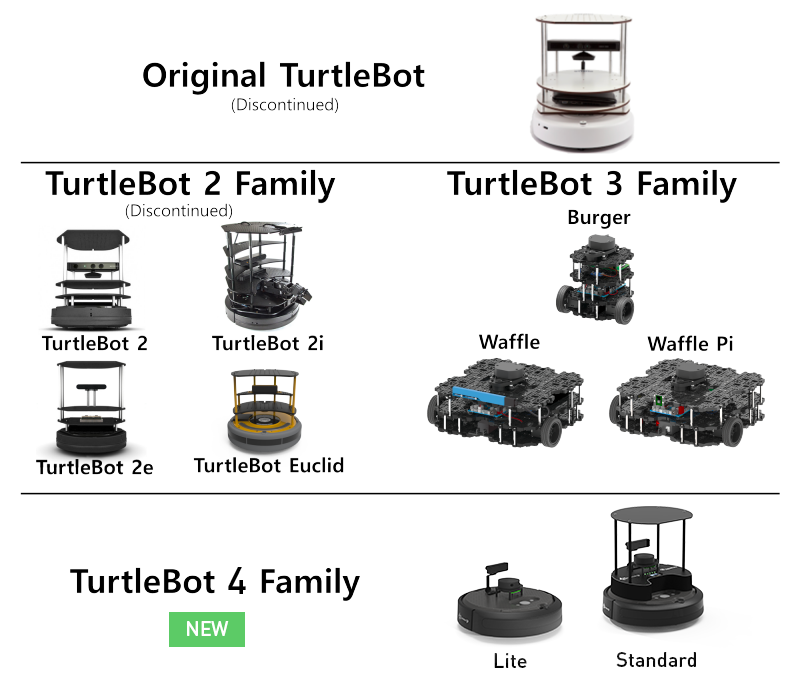
\includegraphics[width=11cm]{figs/turtlebot_family}
  \end{center}
  \caption{Modelos del robot Turtlebot \cite{turtlebot4}}
  \label{fig:turtlebots}
\end{figure}\

\subsection{Turtlebot 2}
\label{sec:turtlebot2}

En concreto, el robot Turtlebot 2\footnote{
\href{https://www.turtlebot.com/turtlebot2/}{https://www.turtlebot.com/turtlebot2/}}
se fundamenta en la base \textit{Kobuki}, que puede verse en la Figura
\ref{fig:base_kobuki}, y que dispone de los sensores necesarios para una
navegación robusta, como puede ser la IMU o Unidad de Medida Inercial, para las
correcciones en los datos de odometría y un \textit{bumper} o sensor de
colisiones.
Esta base \textit{Kobuki} también dispone de una batería que dota al robot de
cierta autonomía y de actuadores que le permiten llevar a cabo dicha navegación,
como son los motores y otros que le permiten transmitir información de manera
visual o auditiva, como los LEDs, y el \textit{buzzer}, con capacidad de
reproducir varios sonidos.
\\

\begin{figure} [h!]
  \begin{center}
    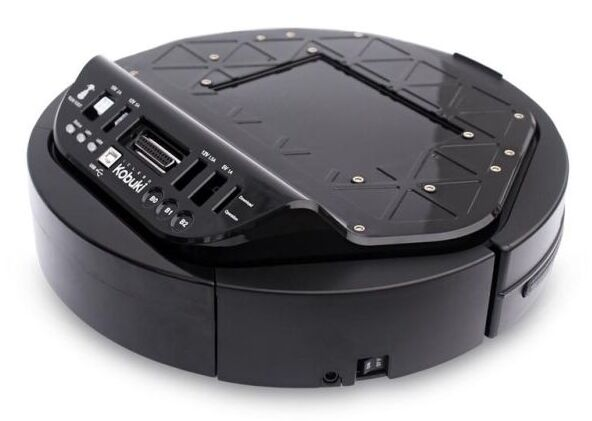
\includegraphics[width=6cm]{figs/kobuki_base}
  \end{center}
  \caption{Base Kobuki \cite{kobuki_base}}
  \label{fig:base_kobuki}
\end{figure}\

Aparte de los componentes de la base, el robot cuenta con una estructura de
madera soportada por barras de aluminio que permite apoyar un ordenador
portátil a modo de ordenador de a bordo, y sensores externos, cuyos modelos
pueden variar dependiendo del robot utilizado en cada momento, ya que se
disponen de varias configuraciones de los mismos en el laboratorio, sin afectar
a la compatibilidad.
Dichos sensores son: un LIDAR para la detección de obstáculos (modelos
RPLIDAR\footnote{\href{https://www.slamtec.ai/product/slamtec-rplidar-s2/?gad_source=1&gclid=CjwKCAjwrIixBhBbEiwACEqDJdjBNB-VeyXLm1hxO33F5wKfJLRu6KRyC1aa4NfaTWvre8dR0scc8xoCMq8QAvD_BwE}{https://www.slamtec.ai/product/slamtec-rplidar-s2/}}
A1 o A2), y una cámara RGBD, de color RGB y profundidad (modelos
Orbbec\footnote{\href{https://www.orbbec.com/}{https://www.orbbec.com/}} Astra o
Asus\footnote{\href{https://www.asus.com/es/}{https://www.asus.com/es/}} Xtion).
Este último sensor aporta un gran potencial debido a su versatilidad en cuanto a
la detección se refiere.
Se puede ver una imagen del modelo en la Figura \ref{fig:turtlebot2}.
\\

\begin{figure} [h!]
  \begin{center}
    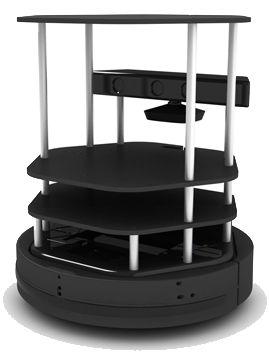
\includegraphics[width=6cm]{figs/turtlebot2}
  \end{center}
  \caption{Turtlebot 2 \cite{turtlebot4}}
  \label{fig:turtlebot2}
\end{figure}\


\subsection{Turtlebot 4}
\label{sec:turtlebot4}

Por su parte, el robot Turtlebot 4\footnote{
\href{https://www.turtlebot.com/}{https://www.turtlebot.com/}} \textit{Lite}
utilizado es bastante parecido al anterior en cuanto a los sensores de la base
se refiere, correspondiendo esta vez con el modelo Create 3 de iRobot\footnote{
\href{https://www.irobot.es/es_ES/roomba.html?gad_source=1&gclid=CjwKCAjwrIixBhBbEiwACEqDJcM6GMOs9Ew0S98K9IJvOaBGm30dR6D1pk5T09dpqwcvNVTaYr7ZTBoC3HgQAvD_BwE}{https://www.irobot.es/es\_ES/roomba.html}}
que, a efectos prácticos, es una aspiradora robótica sin el aspirador ni las
escobillas que las caracterizan, como se puede observar en la Figura
\ref{fig:turtlebot4}.
\\

\begin{figure} [h!]
  \begin{center}
    \includegraphics[width=8cm]{figs/turtlebot4}
  \end{center}
  \caption{Turtlebot 4 \textit{Lite} (izquierda) y \textit{Standard} (derecha) \cite{turtlebot4}}
  \label{fig:turtlebot4}
\end{figure}\

Este robot también añade un sensor LIDAR y una cámara RGBD, que, en el caso de
nuestro laboratorio, son los modelos \textit{RPLIDAR-S2} y \textit{Oak-D-Pro}
respectivamente, sustituyendo a los modelos originales \textit{RPLIDAR-A1} y
\textit{Oak-D-Lite}.
A diferencia de su versión estándar y del anterior robot, este no tiene una
estructura de soporte, por lo que el ordenador de a bordo es una Raspberry
Pi 4 Model B\footnote{
\href{https://www.raspberrypi.com/products/raspberry-pi-4-model-b/}{https://www.raspberrypi.com/products/raspberry-pi-4-model-b/}},
como la mostrada en la anterior Figura \ref{fig:raspberry_pi}, que en nuestro
caso tiene 8Gb de RAM, aunque en el modelo original es de 4Gb.
\\


\subsection{Ordenadores de a bordo}
\label{sec:a_bordo}

Como ya se ha presentado en la Sección \ref{sec:turtlebot2}, para comandar
órdenes al robot se necesita un ordenador de a bordo.
En nuestro caso se ha utilizado un ordenador portátil, de la marca HP, modelo
\textit{ProBook 450 G6}\footnote{
\href{https://support.hp.com/es-es/document/c06195762}{https://support.hp.com/es-es/document/c06195762}},
mostrado en la Figura \ref{fig:hp_probook}.
\\

\begin{figure} [h!]
  \begin{center}
    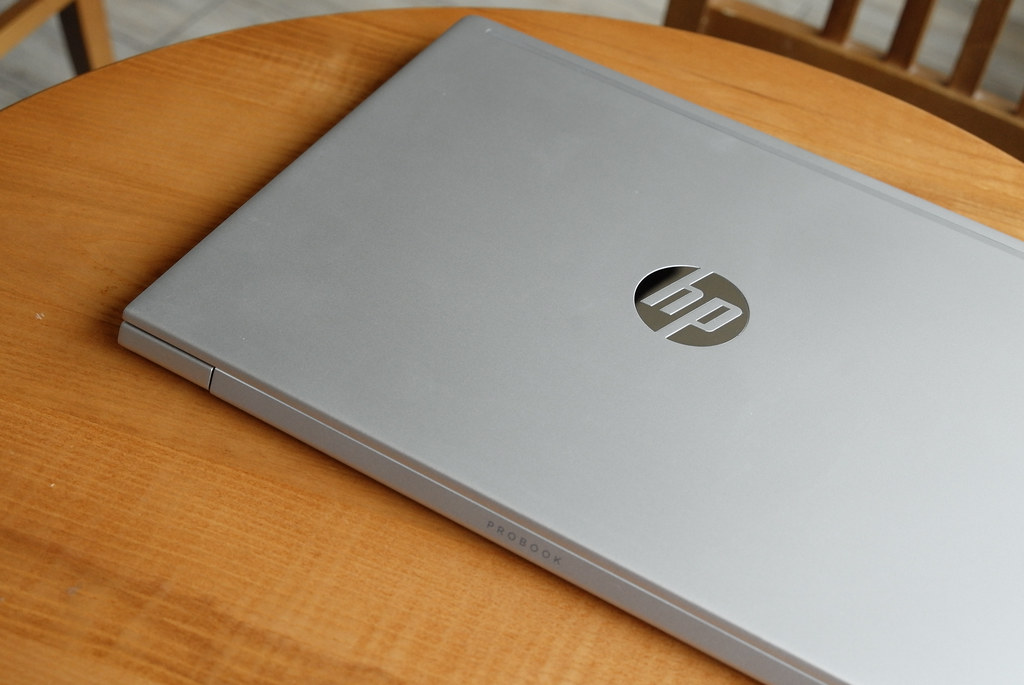
\includegraphics[width=8cm]{figs/hp_probook}
  \end{center}
  \caption{Ordenador portátil HP, modelo ProBook 450 G6 \cite{hp_probook}}
  \label{fig:hp_probook}
\end{figure}\

Para algunas de las pruebas realizadas también se añadió una Raspberry Pi 4
Model B, de 4Gb de RAM, como ordenador de a bordo de uno de los robots Turtlebot
2.
\\

\subsection{Ordenador principal}
\label{sec:ordenador_principal}

Para llevar a cabo este trabajo se precisó de la utilización de un ordenador con
la suficiente capacidad tanto de desarrollar el \textit{software}, como de
llevar a cabo las pruebas del mismo, ejecutando los resultados tanto en un
entorno simulado como en uno real.
Este ordenador también se corresponde con el portátil HP mencionado en la
Sección \ref{sec:a_bordo}.
\\

En cuanto a las pruebas realizadas con robots reales, el uso de este mismo
componente a modo de ordenador principal o centralizado también fue necesario.
Este ordenador portátil es el \textit{hardware} en el que se albergó toda la
capacidad de cómputo acerca de la toma de decisiones, así como el lugar de
ejecución del \textit{software} utilizado para la ejecución de la aplicación
robótica creada.
\\

\subsection{Router}
\label{sec:router}

La comunicación entre los distintos robots es una parte indispensable de este
trabajo, por lo que surge la necesidad de añadir un \textit{hardware} con la
capacidad de comunicar múltiples robots, en nuestro caso un router de la marca
ASUS, Modelo ROG Rapture
GT-AXE16000\footnote{
\href{https://rog.asus.com/es/networking/rog-rapture-gt-axe16000-model/}{https://rog.asus.com/es/networking/rog-rapture-gt-axe16000-model/}}
sin necesidad de conexión a Internet, ya que se utiliza únicamente para la
comunicación local entre los distintos robots, y que se puede observar en la
Figura \ref{fig:asus_router}.
\\

\begin{figure} [h!]
  \begin{center}
    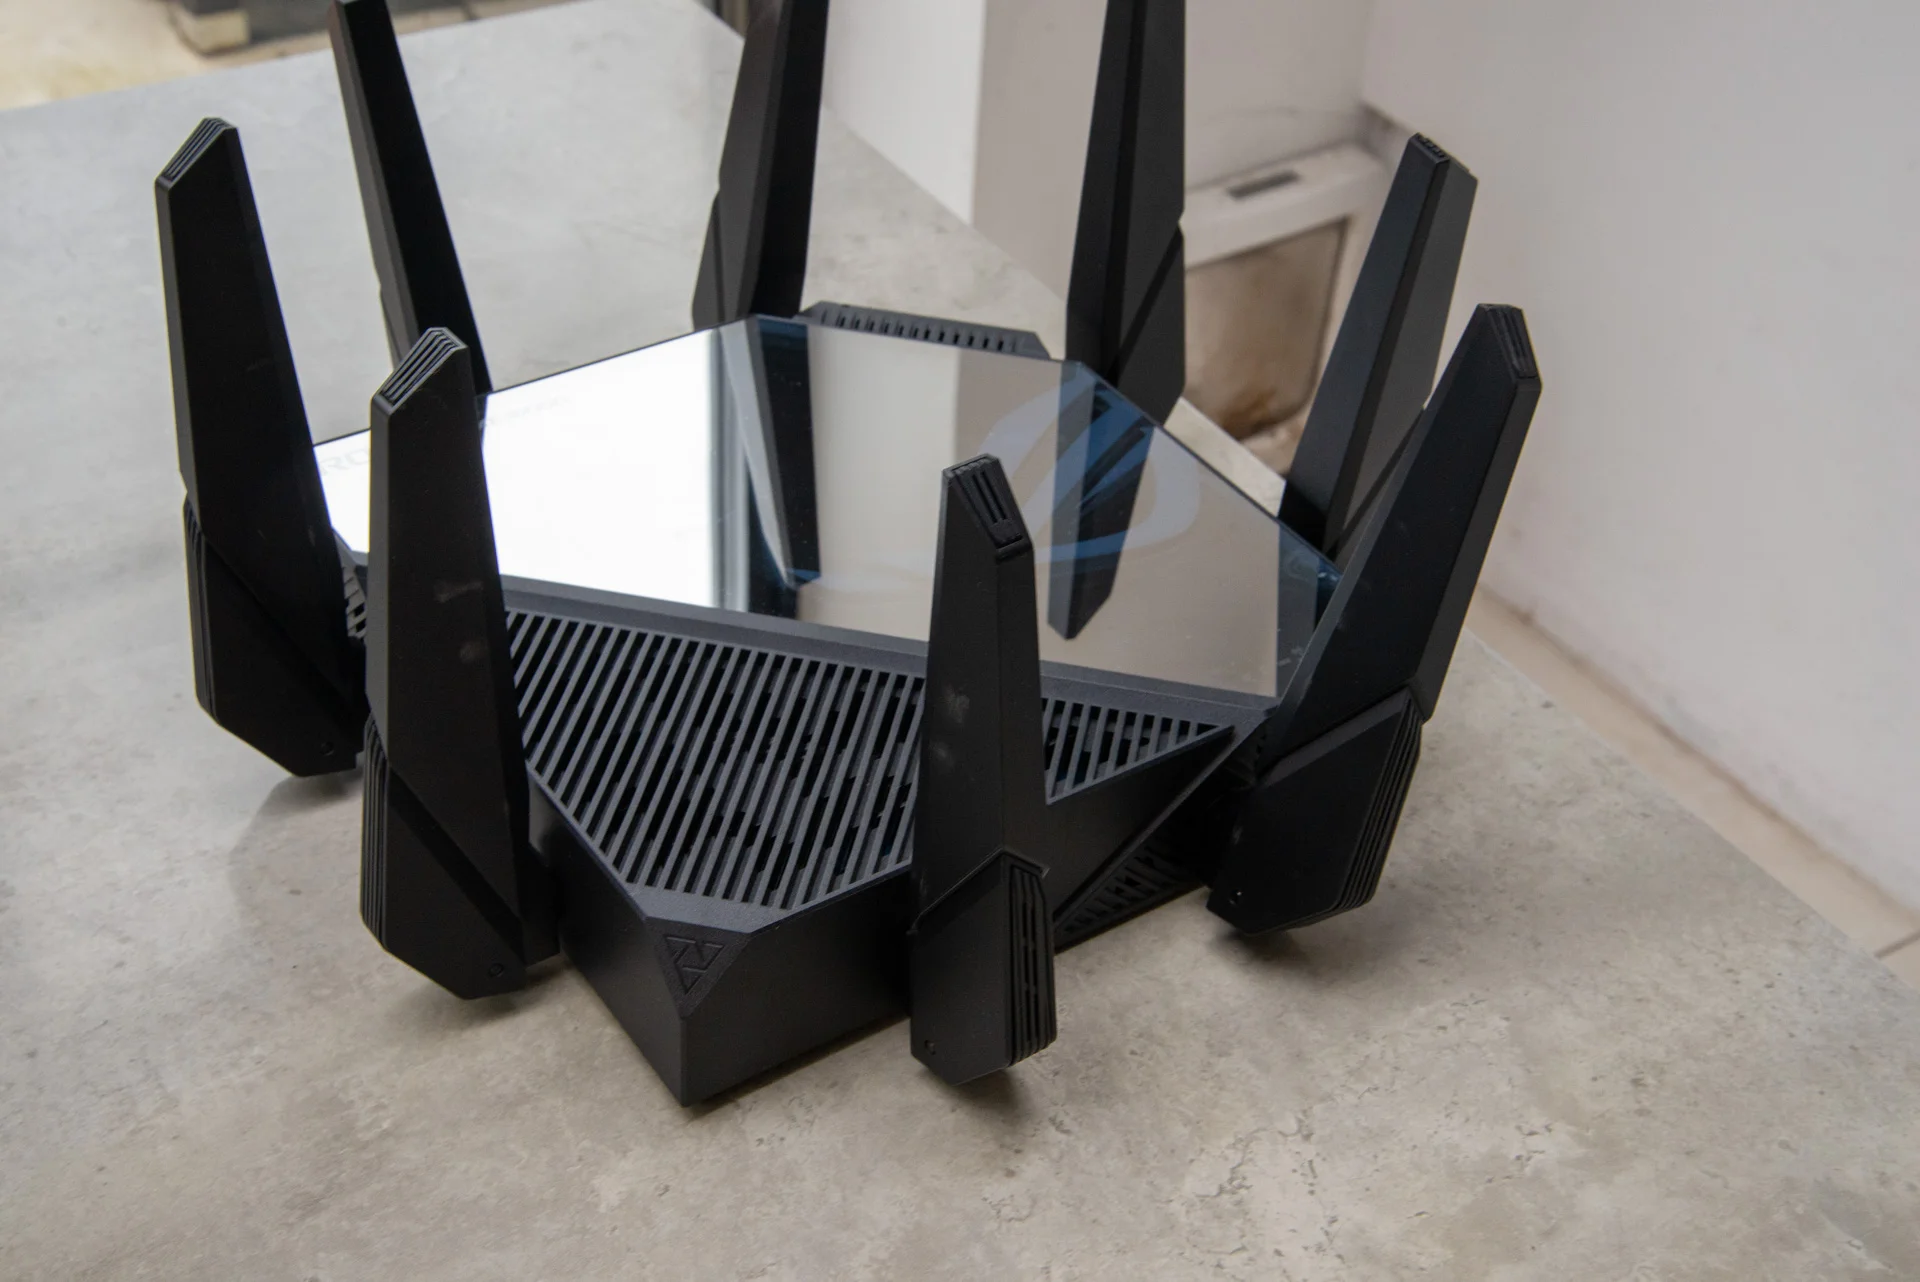
\includegraphics[width=8cm]{figs/asus_router}
  \end{center}
  \caption{Router ASUS, modelo ROG Rapture GT-AXE16000 \cite{asus_router}}
  \label{fig:asus_router}
\end{figure}\


\section{Software}
\label{sec:software}

El \textit{software} desempeña un papel crucial al convertir las capacidades del
\textit{hardware} en acciones concretas.
Es el encargado de emitir las instrucciones necesarias para que el robot, en
conjunto, funcione como un sistema inteligente capaz de llevar a cabo la tarea
definida.
En ausencia de una programación inteligente, el robot permanecerá como un
dispositivo inerte, con un potencial latente pero incapaz de realizar tareas de
manera autónoma.
\\

A continuación se explicarán las distintas herramientas \textit{software}
utilizadas, desde el sistema operativo, pasando por el lenguaje de programación
principal, hasta el \textit{middleware} robótico.
\\


\subsection{Sistema Operativo}
\label{sec:sistema_operativo}

El sistema operativo utilizado es Ubuntu en su versión 22.04 LTS (Long Term
Support o soporte a largo plazo).
Además, es una distribución basada en Debian GNU/Linux, que a su vez se basa en
el \textit{software} libre y de código abierto, lo que permite una mayor
participación de cualquier persona en su desarrollo, aumentando su robustez y
mejorando su soporte.
\\

Esta elección se fundamenta principalmente en la facilidad de uso y programación
con el mismo, así como la compatibilidad con el resto de programas utilizados.
La versión del sistema operativo utilizada coincide con la más nueva de soporte
a largo plazo en la fecha de realización de este proyecto.
\\


\subsection{Lenguaje de programación}
\label{sec:lenguaje_programacion}

El lenguaje de programación utilizado para el desarrollo del \textit{software}
de este trabajo, es \texttt{Python}, ya que debido a su sencillez de
programación y a su legibilidad de código, da lugar a un buen entorno para el
desarrollo de \textit{software} educativo, permitiendo una gran facilidad a la
hora de aprender, además de ser de código abierto, con las respectivas ventajas
que esto supone, explicadas en la Sección \ref{sec:sistema_operativo}.
\\

\texttt{Python} es un lenguaje de programación interpretado, lo que evita tener
que ser compilado, que suele conllevar un proceso tedioso para programadores
principiantes.
Además, se define como lenguaje de alto nivel, ya que soporta la programación
orientada a objetos (OOP), lo que también permite su escala en complejidad, si
así se requiriese.
\\

Este lenguaje ha tomado un gran impulso en los últimos años debido a su
popularidad, aunque cabe destacar que es un lenguaje sumamente lento en
comparación a otros más simples, y generalmente de más bajo nivel, como
\texttt{C}.
En concreto utilizaremos la versión 3 de este lenguaje debido a su
compatibilidad y a su relevancia actual.
\\

Este lenguaje de programación será usado directamente a la hora de programar
nuestro propio \textit{software}.
Además, otros lenguajes serán utilizados indirectamente por aplicaciones o nodos
externos.
Por ejemplo, \texttt{C++} será utilizado en algunos nodos de ROS2, mientras que
\texttt{Rust}, un lenguaje con una creciente popularidad y conocido por su
seguridad y rendimiento, además de su excelente gestión de la memoria, estará
presente en los programas relacionados con Zenoh.
\\

\subsection{Middleware Robótico}
\label{sec:middleware_robotico}

%Párrafo sobre ROS2
ROS2 es un \textit{middleware} robótico creado para abstraer al programador del
\textit{hardware} del robot, permitiendo una mayor atención en el desarrollo
\textit{software} del mismo.
Por todo ello, simplifica este proceso, sirviendo de herramienta tanto para la
programación o desarrollo, como para el uso o la ejecución del \textit{software}
en cuestión.
\\

En este \textit{middleware}, el código se divide en nodos ejecutables de manera
iterativa a una determinada frecuencia, que pueden comunicarse a través del
protocolo DDS, generalmente con la utilización de \textit{topics}, ya que dicho
protocolo basa su funcionamiento en un modelo de publicador/suscriptor, donde
los componentes del sistema se dividen en publicadores, responsables de enviar
datos, y suscriptores, encargados de recibirlos.
La comunicación se facilita mediante un \textit{broker} o intermediario, que
coordina la trasferencia de mensajes entre los nodos, permitiendo una
comunicación flexible y organizada en temas anteriormente llamados
\textit{topics}, y sin necesidad requerir que los publicadores y suscriptores
se conozcan directamente.
La librería cliente de ROS2 permite programar los nodos en \texttt{Python} o
\texttt{C++}, aunque la amplia comunidad ha desarrollado extraoficialmente el
equivalente en otros lenguajes como \texttt{Java}, \texttt{C}, \texttt{Rust} o
incluso \texttt{Android}, entre otros.
\\


\subsection{Simulación}
\label{sec:simulacion}

%Párrafo sobre Gazebo y lenguajes de marcado tipo XML como URDF/SDF
En cuanto a la simulación, el \textit{software} utilizado es Gazebo, un
simulador muy popular que permite la visualización de los robots y de los
entornos, gracias a su previa descripción, generalmente mediante un archivo con
formato XML (eXtensible Markup Language) o derivado, que pueden ser
URDF\footnote{\href{https://wiki.ros.org/urdf}{https://wiki.ros.org/urdf}}
(Unified Robotics Description Format) y SDF\footnote{
\href{http://sdformat.org/}{http://sdformat.org/}} (Simulation Description
Format) respectivamente.
Puede verse un ejemplo de simulación en la Figura \ref{fig:gazebo_sim}.
\\

\begin{figure} [h!]
  \begin{center}
    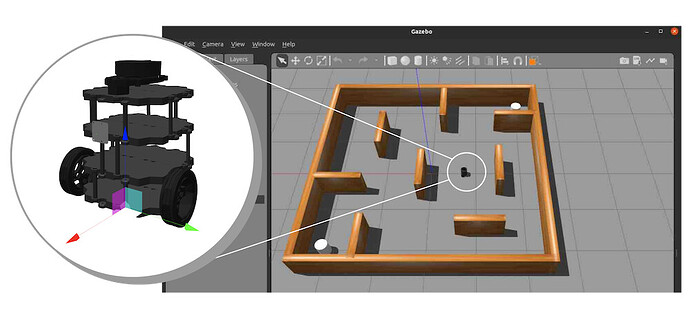
\includegraphics[width=10cm]{figs/gazebo_sim}
  \end{center}
  \caption{Gazebo simulando un robot Turtlebot 3 en un mundo virtual \cite{gazebo}}
  \label{fig:gazebo_sim}
\end{figure}\

Este simulador también permite la visualización de ciertos datos de sus sensores
si así se requiere, o de las partes o componentes de un robot gracias al archivo
de descripción del mismo, mencionado en el párrafo anterior.
Además permite el uso de \textit{plugins} que pueden añadir las funcionalidades
que sean necesarias.
\\


\subsection{Protocolos de comunicación}
\label{sec:protocolos_comunicacion}

%%% [Párrafo sobre ZettaScale y sus softwares utilizados]
En este ámbito, una de las empresas más importantes es ZettaScale
Technology\footnote{
\href{https://www.zettascale.tech/}{https://www.zettascale.tech/}}, que ha
tomado mucha relevancia en los últimos años, ya que es responsable de una de las
implementaciones de \textit{middleware} de telecomunicaciones de DDS utilizado
en ROS2, llamado CycloneDDS\footnote{
\href{https://cyclonedds.io/}{https://cyclonedds.io/}}, y son los
desarrolladores de un reciente protocolo de comunicaciones llamado
Zenoh\footnote{\href{https://zenoh.io/}{https://zenoh.io/}} \cite{zenoh}, por
sus siglas en inglés, Zero Overhead Network Protocol, que ya cuenta con
importantes clientes, como la NASA, debido a las prestaciones que este ofrece,
superando en la mayoría de casos a los protocolos de su misma índole y que ya ha
sido oficialmente seleccionado como el próximo RMW (ROS \textit{Middleware} o
\textit{Middleware} de comunicación de ROS) de ROS2\footnote{
\href{https://discourse.ros.org/t/ros-2-alternative-middleware-report/33771}{https://discourse.ros.org/t/ros-2-alternative-middleware-report/33771}}.
El protocolo Zenoh, está basado en un modelo de publicador/suscriptor, así como
DDS, por lo que hacen una buena sinergia.
\\

Además de esto, poseen un potente \textit{framework} para la programación de
flujos de datos aún en desarrollo, llamado
Zenoh-Flow\footnote{
\href{https://zenoh.io/blog/2023-02-10-zenoh-flow/}{https://zenoh.io/blog/2023-02-10-zenoh-flow/}},
\cite{zenohflow} así como un puente llamado Zenoh-Bridge-DDS\footnote{
\href{https://github.com/eclipse-zenoh/zenoh-plugin-dds}{https://github.com/eclipse-zenoh/zenoh-plugin-dds}}
que hace las veces de traductor entre los protocolos DDS y Zenoh, lo que permite
la comunicación entre estos flujos de datos con nodos de ROS2, haciendo posible
la creación de aplicaciones robóticas en forma de flujos de datos, utilizando
nodos de ROS2 existentes, y fusionando de esta manera ambos campos.
\\

Es notable destacar el gran soporte que brinda esta empresa, que ayuda en gran
medida a resolver los problemas o dudas que puedan surgir durante el desarrollo o
despliegue de las aplicaciones.
\\

El protocolo de comunicaciones utilizado en el \textit{software} desarrollado en
este trabajo es Zenoh, que reduce en gran medida los bytes de la cabecera de los
mensajes, y ofrece mejores prestaciones en comparación con otros protocolos de
su misma índole, como se puede apreciar en la gráfica de la Figura
\ref{fig:zenoh_performance}, del artículo \cite{liang2023zenoh_performance} en
el que se hicieron distintas pruebas, una de ellas en varias máquinas,
con los protocolos Kafka, MQTT, CycloneDDS y distintas variantes de Zenoh,
siendo estas últimas las que mejores resultados obtuvieron, en esta como en las
demás pruebas.
\\

\begin{figure} [h!]
  \begin{center}
    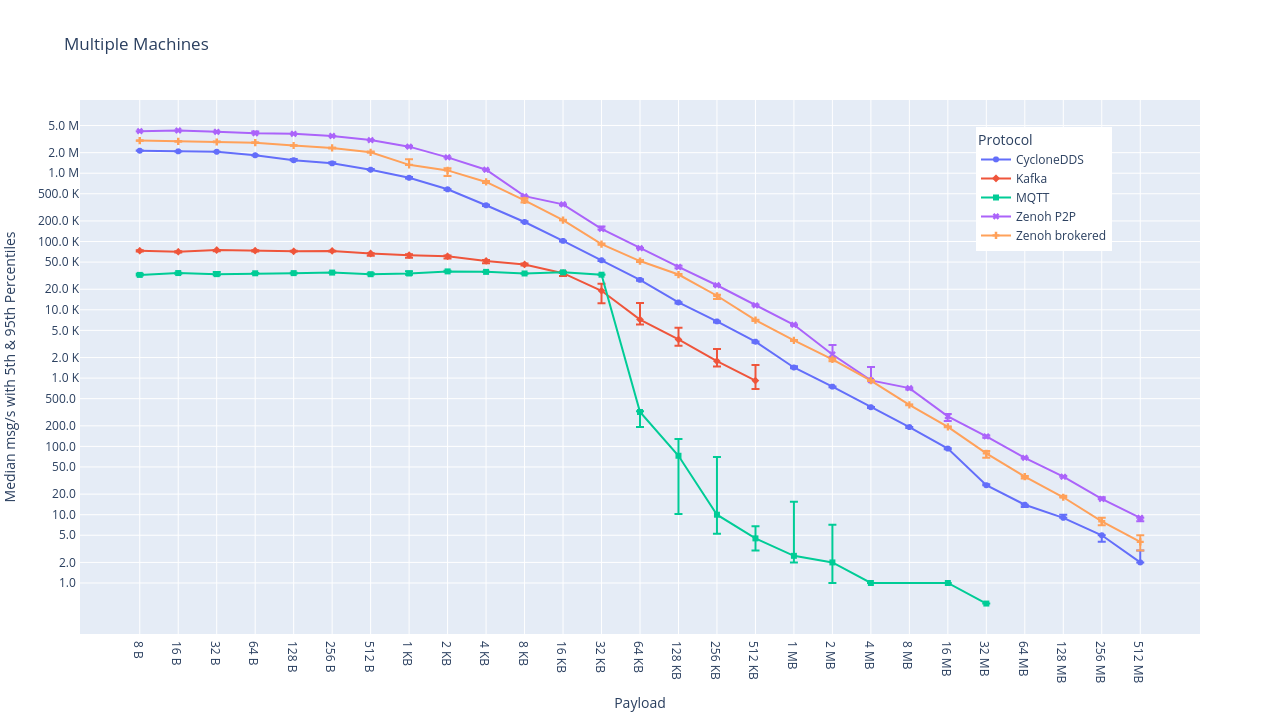
\includegraphics[width=15cm]{figs/zenoh_performance}
  \end{center}
  \caption{Rendimiento de distintos protocolos \cite{zenoh_performance}.}
  \label{fig:zenoh_performance}
\end{figure}\

En nuestro caso utilizaremos Zenoh-Flow para la programación de flujos de datos,
ya que tiene una API (Application Programming Interface) en \texttt{Python}, lo
que permite programarlos de manera sencilla, como se ha explicado en la Sección
\ref{sec:lenguaje_programacion}.
\\

También se utilizará DDS indirectamente en los nodos de ROS2 de los que se hará
uso, para los que utilizaremos la RMW de CycloneDDS, ya que es el que mejor
funciona con el software utilizado.
\\

Además, enlazaremos dichos nodos de ROS2 con nuestro flujo de datos mediante el
uso del Zenoh-Bridge-DDS, que nos permitirá traducir los mensajes de un
protocolo a otro en ambos sentidos, ya que Zenoh-Flow utiliza Zenoh para las
comunicaciones, mientras que ROS2 se comunica mediante DDS.
\\


\subsection{Visión Artificial}
\label{sec:vision_artificial}

Para la detección de objetos a partir de imágenes, ya sean generadas por una
cámara o creadas a partir de los datos de otros sensores, se ha utilizado una
reconocida librería de procesamiento de imágenes llamada OpenCV, disponible
tanto en \texttt{Python} como en \texttt{C++}.
\\

Este software permite, entre otras muchas cosas, el cambio entre distintos
espacios de color, entre los que se encuentran los formatos RGB, GreyScale o
escala de grises, que permite ahorrar memoria o detectar bordes o HSV (Hue,
Saturation, Value), que permite entre otros muchos usos, trabajar con los
colores en distintas intensidades de luz, brindando así mejores resultados que
con otros espacios de color.
Este espacio de color se ve representado en la Figura \ref{fig:hsv}.
\\

\begin{figure} [h!]
  \begin{center}
    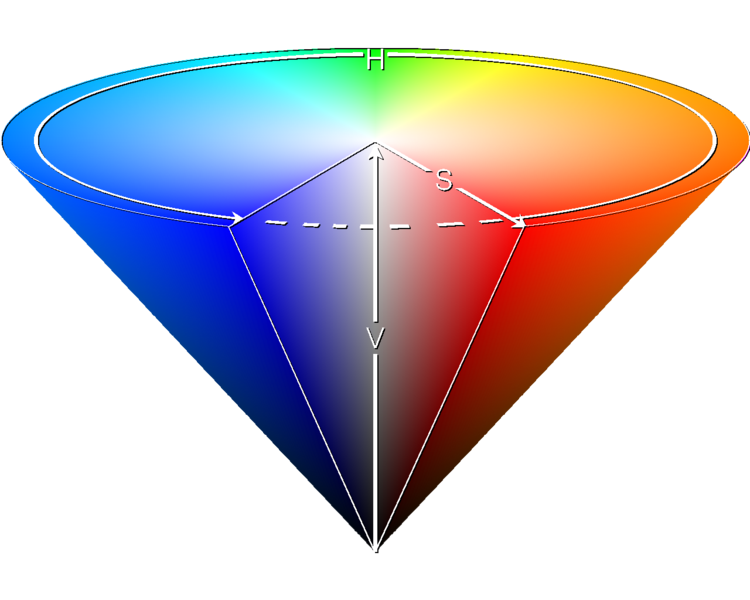
\includegraphics[width=6cm]{figs/hsv_cone}
  \end{center}
  \caption{Espacio de color HSV \cite{hsv_cone}}
  \label{fig:hsv}
\end{figure}\

Esta librería también ofrece distintas funciones de detección, como pueden ser
la detección de rostros, bordes o contornos, o la detección de objetos mediante
aprendizaje profundo.
En nuestro caso se han utilizado, tanto la detección de objetos mediante el uso
de un filtro de color aplicado a la imagen obtenida desde la cámara, como la
detección de bordes en conjunto con la posterior detección de círculos, en una
imagen generada a partir de los datos posicionales de un sensor LIDAR, como se
explicará en la Sección \ref{sec:pruebas_app}.
\\

Esta librería también se apoya en otra, llamada Numpy, encargada de la
representación matemática eficiente de matrices, así como de operaciones
matemáticas entre ellas, ya que las imágenes a color, generalmente son matrices
tridimensionales, que albergan tres canales (RGB o HSV), cuyas columnas tienen
el tamaño de la longitud vertical de la imagen en píxeles, así como el tamaño de
las filas, corresponde con el ancho de la imagen, como se puede ver en la Figura
\ref{fig:rgb_mat}.
\\

\begin{figure} [h!]
  \begin{center}
    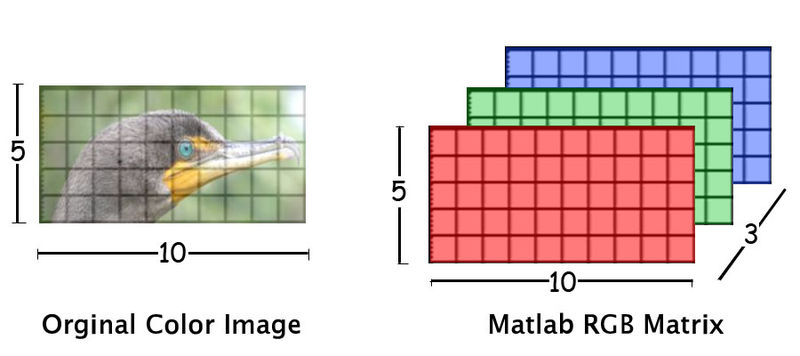
\includegraphics[width=10cm]{figs/rgb_matrix}
  \end{center}
  \caption{Representación de imagen RGB como matriz \cite{rgb_mat}}
  \label{fig:rgb_mat}
\end{figure}\


\subsection{Software de navegación}
\label{sec:navegacion}

El \textit{software} de navegación utilizado para trasladar los robots de una
posición a otra en el espacio se basa en los paquetes del conocido
\textit{stack} de Nav2\footnote{
\href{https://github.com/ros-navigation/navigation2}{https://github.com/ros-navigation/navigation2}},
que brinda herramientas que solucionan la navegación del robot de manera
bastante robusta y precisa, gracias a un método de localización probabilístico
basado en el algoritmo de Montecarlo.
Este algoritmo consiste en distribuir una gran cantidad de puntos a lo largo del
mapa del entorno, que representan posibles ubicaciones del robot, y por tanto se
moverán de acuerdo al movimiento del mismo.
Además, tienen una probabilidad asociada basada en los datos de los sensores,
alrededor de la cual se desarrollará una nueva generación de partículas: se
partirá de las más probables añadiendo una variable de aleatoriedad y se
eliminarán las de menor probabilidad, acercándose de esta manera en cada
iteración a la posición real del robot, incluso en entornos altamente
simétricos.
\\


\subsection{Software matemático}
\label{sec:software_matematico}
%librerias Numpy, Math, y las transformadas de ROS2.

Para suplir la necesidad de realizar operaciones matemáticas de todo tipo, como
pueden ser las transformaciones entre espacios de coordenadas o entre ejes de
coordenadas, operaciones simples o complejas con grandes cantidades de números,
como matrices o imágenes, o cualquier otro tipo de operaciones, se han utilizado
tanto la librería Numpy como Math, dependiendo del tipo de operación, ya que
ambas son muy eficientes.
\\

Para operaciones de transformadas (TFs) de ROS2 entre dos \textit{frames},
utilizaremos las propias herramientas de ROS2, aunque no podremos utilizar
cualquiera, ya que la mayoría tienen la necesidad de correr en un nodo de ROS2
y no funcionan fuera del mismo, por lo que concretamente utilizaremos la
función del Código \ref{cod:code_tfs}.
Es por lo que se necesitará haber creado una suscripción previamente al
\textit{topic} de TFs del robot en cuestión.
\\

\begin{code}[h!]
  \begin{lstlisting}[language=Python]
    from builtin_interfaces.msg import Duration
    import tf2_ros, rclpy

    buffer_core = tf2_ros.BufferCore(Duration(sec=1, nanosec=0))
    buffer_core.lookup_transform_core(
      frame_id_1, frame_id_2, rclpy.time.Time()
      )
  \end{lstlisting}
  \caption[Función para calcular transformadas]{Función para calcular transformadas (TFs)}
  \label{cod:code_tfs}
\end{code}


\subsection{Visualización de datos}
\label{sec:visualizacion_datos}

Para representar de manera simplificada y visual todos los datos, tanto de los
sensores como de los actuadores de los robots, se utiliza
RViz2\footnote{
\href{https://github.com/ros2/rviz}{https://github.com/ros2/rviz}}, una
herramienta integrada en ROS2 que permite visualizar imágenes procedentes de las
cámaras, así como el propio modelo del robot en movimiento, o la posición
probabilística del mismo derivada de un algoritmo de localización, como el
mencionado en la Sección \ref{sec:navegacion}.
\\

Además, a la hora de hacer pruebas, también se han usado otras herramientas, como
la misma librería de OpenCV, para crear ventanas que muestran una imagen con
\textit{sliders} que permiten modificar variables, generando de esta manera una
mayor interactividad y fluidez a la hora de encontrar los valores óptimos de
ciertos parámetros, como pueden ser los valores máximos y mínimos de un filtro
de color, permitiendo ver el resultado en la imagen de manera dinámica, como se
puede observar en la Figura \ref{fig:opencv}.
\\

\begin{figure} [h!]
  \begin{center}
    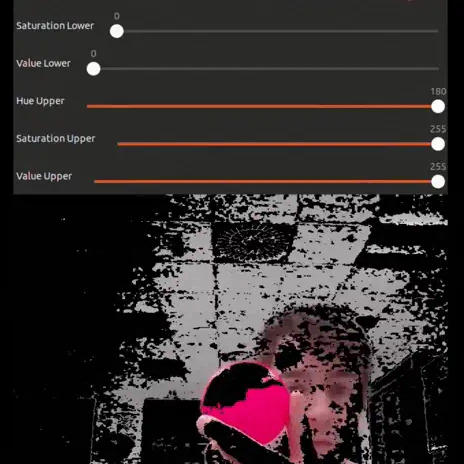
\includegraphics[width=8cm]{figs/opencv_visualization}
  \end{center}
  \caption{\textit{Sliders} de un filtro de color con OpenCV.}
  \label{fig:opencv}
\end{figure}\

Asimismo, se ha utilizado software externo, como
PlotJuggler\footnote{\href{https://plotjuggler.io/}{https://plotjuggler.io/}},
para mostrar gráficas sobre datos provenientes de \textit{topics} en directo.




\chapter{Arquitectura software}
\label{cap:capitulo4}

\begin{flushright}
%\begin{minipage}[]{10cm}
\emph{La práctica es el único camino para la maestría.}\\
%\end{minipage}\\

Stephen R. Covey, \textit{Los 7 hábitos de la gente altamente efectiva}\\
\end{flushright}

\vspace{1cm}

%Escribe aquí un párrafo explicando brevemente lo que vas a contar en este capítulo. En este capítulo (y quizás alguno más) es donde, por fin, describes detalladamente qué has hecho y qué experimentos has llevado a cabo para validar tus desarrollos.

Este capítulo describe la topología de red utilizada, tanto a nivel de
\textit{hardware} como a nivel de \textit{software}.
También se describe la manera en la que los distintos elementos
\textit{software} se complementan, detallando los aspectos más importantes de
cada uno de ellos, y explicando cómo funcionan juntos.



\section{Topología hardware}
\label{sec:topologia_hw}

%párrafo sobre la topología harware de red
La topología de red utilizada comprende varias máquinas, debido a la naturaleza
multirobótica de este trabajo, correspondiendo todas ellas, a los ordenadores de
a bordo de los robots utilizados, a excepción del \textit{router}, que será el
componente encargado de establecer comunicaciones entre el resto de máquinas y
encaminar así los datos que se envían entre ellas.
\\

%párrafo sobre el router a nivel harware y configuración (software).
Comenzando con el \textit{router}, podemos remarcar que no se ha necesitado una
conexión a internet, ya que las comunicaciones se han realizado de manera local,
es decir, que todos los ordenadores de abordo en los robots se comunican
directamente con dicho \textit{router}, sin necesidad de mandar datos más allá
de esta red local, dado que todos se encuentran en la misma sala, al alcance de
un único \textit{router}.
Asimismo este debe estar configurado de manera que permita la comunicación en
ambos sentidos (entrante y saliente), y debe permitirla a través de los
protocolos DDS, para los nodos de ROS2; y Zenoh, para los nodos de Zenoh-Flow.
\\

%párrafo sobre los ordenadores de a bordo de los robots.
Los ordenadores de a bordo deben tener una mínima capacidad de cómputo como para
no saturarse a la hora de enviar o recibir una gran cantidad de mensajes.
En nuestro caso se ha utilizado el ordenador portátil mencionado en la Sección
\ref{sec:a_bordo}.
Puesto que se necesitan más ordenadores para realizar los experimentos, y solo
se dispone de un ordenador portátil, también se han utilizado las máquinas del
modelo Raspberry Pi 4B mencionadas en la sección referenciada.
\\

\begin{figure} [h!]
  \begin{center}
    \includegraphics[width=8cm]{figs/network_topology}
  \end{center}
  \caption{Topología de red centralizada.}
  \label{fig:network_topology}
\end{figure}\

El ordenador portátil se ha utilizado en conjunto con el robot Turtlebot 2,
mostrado en la Sección \ref{sec:turtlebot2}, mientras que las Raspberry Pi 4B es
utilizada en los propios robots Turtlebot 4, mostrados en la Sección
\ref{sec:turtlebot4}, a modo de ordenador de a bordo interno.
\\

Dado que el portátil es el ordenador más potente utilizado, este deberá correr
todo el software relativo a Zenoh-Flow, además de estar conectado al robot, como
se puede ver representado en la Figura \ref{fig:network_topology}.
\\



\section{Topología software}
\label{sec:topologia_sw}

%párrafo sobre los ordenadores de a bordo de los robots.
A nivel de \textit{software}, aparte de la configuración del \textit{router}
mencionada anteriormente, se ha necesitado ejecutar un \textit{router} de Zenoh
y un \textit{bridge} de Zenoh en cada robot, permitiendo de esta manera las
comunicaciones en ambos sentidos entre ellos y a su vez la utilización de los
protocolos Zenoh y DDS al mismo tiempo.
Las máquinas utilizadas también necesitan una configuración de red para poder
operar con estas herramientas \textit{software}.
\\

Además, nuestra topología será centralizada, lo que quiere decir que una de las
máquinas, llamada ordenador principal o centralizado, correrá todo el
\textit{software} desarrollado en Zenoh-Flow, por lo que deberá tener instalado
dicho \textit{software} además del \textit{router} y del bridge de Zenoh.
La máquina elegida para este propósito será consecuentemente la que mayor
capacidad de cómputo tiene, que en este caso es el portátil, como se ha
mencionado en la Sección \ref{sec:topologia_hw}.


\subsection{Zenoh-bridge-DDS}
\label{sec:zenoh_bridge}

Como ya se ha mencionado previamente, este \textit{software} permite traducir
las comunicaciones entre Zenoh y DDS, en ambas direcciones, estableciendo un
puente entre ellas, como su nombre indica.
Gracias a esta propiedad del \textit{bridge} y a la posibilidad de serializar
los mensajes en el interior de los nodos de Zenoh-Flow, utilizando la misma
función que se usa internamente en ROS2 para serializarlos, se puede establecer
una comunicación directa entre nodos de Zenoh-Flow y de ROS2 en ambas
direcciones y a pesar de utilizar distintos protocolos.
\\

Esto nos permite seguir utilizando las funcionalidades existentes programadas
en ROS2, a la vez que desarrollar código compatible en Zenoh-Flow que utilice
dichas funcionalidades sin ningún impedimento, como se verá más adelante en la
Sección \ref{sec:zenoh_flow}.
\\


\subsection{Zenoh-Flow}
\label{sec:zenoh_flow}

Zenoh-Flow es un \textit{framework} diseñado para la programación de flujos de
datos, que funciona sobre el protocolo Zenoh, y que se puede comunicar a través
de DDS con nodos de ROS gracias al Zenoh-bridge-DDS, como queda explicado en la
Sección \ref{sec:zenoh_bridge}.
Esta capacidad nos permite hacer uso de nodos de ROS en los flujos de datos, así
como realizar aplicaciones robóticas directamente en conjunto con nodos de ROS,
como se explica más adelante en esta sección.
\\

Para la programación de flujos de datos con este \textit{framework} es necesario
la definición de un flujo de datos, en un archivo en formato \texttt{yaml}, como
el que podemos ver en el ejemplo del Código \ref{cod:data_flow_example} y que
puede encontrarse en el repositorio oficial de ejemplos de Zenoh-Flow\footnote{
\href{https://github.com/ZettaScaleLabs/zenoh-flow-examples/blob/master/getting-started}{https://github.com/ZettaScaleLabs/zenoh-flow-examples/blob/master/getting-started}}.
\\

% Con esta linea no funciona (para usar la definición comentada en estilo.tex):
%\begin{lstlisting}[language=yaml]
\begin{code}[h!]
  \begin{lstlisting}[style=yaml]
    flow: getting-started
    vars:
     BASE_DIR: "/path/to/zenoh-flow-examples/getting-started"
    
    sources:
      - id: zenoh-sub
        configuration:
          key-expressions:
            out: zf/getting-started/hello
        descriptor: "builtin://zenoh"
    operators:
      - id: greetings-maker
      descriptor: "file://{{ BASE_DIR }}/nodes/python/greetings-maker/greetings-maker.yaml"
    sinks:
      - id: file-writer
      descriptor: "file://{{ BASE_DIR }}/nodes/python/file-writer/file-writer.yaml"
      - id: zenoh-writer
        configuration:
          key-expressions:
            in: zf/getting-started/greeting
        descriptor: "builtin://zenoh"
    
    links:
      - from:
          node: zenoh-sub
          output: out
        to:
          node: greetings-maker
          input: name
      - from:
          node: greetings-maker
          output: greeting
        to:
          node: file-writer
          input: in
      - from:
          node: greetings-maker
          output: greeting
        to:
          node: zenoh-writer
          input: in
  \end{lstlisting}
\caption[Definición de flujo de datos en Zenoh-Flow]{Definición de flujo de datos en Zenoh-Flow}
\label{cod:data_flow_example}
\end{code}

%Párrafo sobre las etiquetas importantes del código.
En el contenido de este archivo pueden verse varios apartados importantes, como
son: las variables de configuración que recibirán los nodos, denominada con la
etiqueta \verb|vars|; la definición de los distintos nodos con las etiquetas
\verb|source|, \verb|operator| o \verb|sink|, donde se definen las rutas a los
archivos \texttt{yaml} que los describen, incluyendo sus entradas, salidas o
variables de configuración, como se explicarán a continuación; y las conexiones
entre ellos con la etiqueta \verb|links|, en cuyo interior se definen las
conexiones entre las entradas y salidas de cada nodo.
\\

%Párrafo sobre las etiquetas importantes que no están en el código.
Además, se puede añadir la etiqueta \verb|mapping|, donde se especifica en qué
máquina correrá cada nodo, aunque en nuestro caso no será necesario debido a que
todos los nodos correrán en el mismo ordenador (el más potente), para liberar
capacidad de cómputo a los demás.
De esta manera, nuestra topología será centralizada.
\\

%Párrafo sobre los descriptores builtin o integrados.
En este ejemplo se puede ver cómo los nodos \verb|zenoh-sub| y
\verb|zenoh-writer| contienen la línea \verb|descriptor: "builtin://zenoh"|, lo
que indica que no necesitan un fichero que describa dónde se encuentra el código
de dicho nodo, ya que este se encuentra directamente integrado en Zenoh-Flow, y
lo que harán será recibir y información de la \textit{key-expression}
\verb|zf/getting-started/hello| y publicar información a la
\textit{key-expression} \verb|zf/getting-started/greeting| respectivamente, como
puede observarse resumidamente en la Figura \ref{fig:zf_example}.
\\

\begin{figure} [h!]
  \begin{center}
    \includegraphics[width=15cm]{figs/zenoh_flow_example}
  \end{center}
  \caption{Flujo de datos de ejemplo en Zenoh-Flow.}
  \label{fig:zf_example}
\end{figure}\

%Párrafo sobre los descriptores no integrados.
El resto de nodos deben ser programados, para lo que existe un fichero
descriptor, que indicará el nombre del nodo, las variables de configuración, la
ruta al archivo de código del propio nodo y los nombres de sus \textit{inputs} y
\textit{outputs}.
Continuando con el mismo ejemplo, se muestran en el Código
\ref{cod:node_descriptor} las propiedades mencionadas, en este caso del nodo
\textit{operator} con el nombre \verb|greetings-maker|, que consecuentemente se
encontrará en la ruta declarada en su etiqueta \verb|descriptor|.
\\

\begin{code}[h!]
  \begin{lstlisting}[style=yaml]
    id: greetings-maker
    vars:
      BASE_DIR: "/path/to/zenoh-flow-examples/getting-started"
    uri: "file://{{ BASE_DIR }}/nodes/python/greetings-maker/greetings-maker.py"
    inputs: [name]
    outputs: [greeting]
  \end{lstlisting}
\caption[Fichero de descriptor de un nodo de Zenoh-Flow]{Fichero de descriptor de un nodo de Zenoh-Flow}
\label{cod:node_descriptor}
\end{code}

%Párrafo sobre las partes del código del nodo operator de ejemplo.
Las distintas partes del código de este nodo se muestran en el Código
\ref{cod:operator_node}, en el que puede verse cómo se reduce a una sencilla
clase que hereda de la clase del nodo en cuestión, en este caso de la clase
\verb|Operator|. Además debe existir una función externa \verb|register()| que
debe devolver la clase creada para este nodo, en nuestro caso llamada
\verb|GreetingsMaker|.
\\

\begin{code}[h!]
  \begin{lstlisting}[language=Python]
    from zenoh_flow.interfaces import Operator
    from zenoh_flow import Inputs, Outputs
    from zenoh_flow.types import Context
    from typing import Dict, Any
    
    class GreetingsMaker(Operator):
        def __init__(
            self,
            context: Context,
            configuration: Dict[str, Any],
            inputs: Inputs,
            outputs: Outputs,
        ):
            self.output = outputs.take("greeting", str, lambda s: bytes(s, "utf-8"))
            self.in_stream = inputs.take("name", str, lambda buf: buf.decode("utf-8"))
            if self.in_stream is None:
                raise ValueError("No input 'name' found")
            if self.output is None:
                raise ValueError("No output 'greeting' found")
    
        def finalize(self) -> None:
            return None
    
        async def iteration(self) -> None:
            message = await self.in_stream.recv()
            name = message.get_data()
            if name is not None:
                greetings = self.generate_greetings(name)
                await self.output.send(greetings)
            return None
    
        def generate_greetings(self, name: str) -> str:
            greetings_dict = {
                "Sofia": "Ciao, {}!\n",
                "Gabriele": "Ciao, PaaS manager!\n",
            }
            greet = greetings_dict.get(name, "Hello, {}!\n")
            return greet.format(name)
    
    def register():
        return GreetingsMaker
  \end{lstlisting}
\caption[Fichero de código de un nodo \texttt{operator} en Zenoh-Flow]{Fichero de código de un nodo \texttt{operator} de Zenoh-Flow}
\label{cod:operator_node}
\end{code}

La programación de los nodos de Zenoh-Flow, realizada en \texttt{Python}, es muy
parecida entre los distintos nodos, ya que su funcionamiento es muy similar: los
nodos \textit{source} solo comprenden salidas de datos, los nodos \textit{sink}
solo comprenden entradas, y los nodos \textit{operator} comprenden ambas, ya que
pueden recibir información de otros nodos \textit{source} u \textit{operator} y
pueden enviar datos a otros nodos \textit{operator} o \textit{sink}, como
podemos ver en el flujo de datos representado en la anterior Figura
\ref{fig:zf_example} o en la Figura \ref{fig:data_flow_qr_example} de la Sección
\ref{sec:flujos_datos}.
\\

%Párrafos sobre la función constructor (__init__()) de la clase del nodo.
La línea \verb|outputs.take("greeting", str, lambda s: bytes(s, "utf-8"))|, en
la función constructor de esta clase (\verb|__init__()|), toma como argumentos
el nombre del \textit{output}, el tipo de mensaje, y la función que utilizará
para serializar el mensaje en el momento de enviarlo, devolviendo el
\textit{output} correspondiente.
Lo mismo sucede con la línea siguiente, aunque al tratarse de un \textit{input},
esta toma como tercer argumento una función que utilizará para deserializar el
mensaje en el momento en el que sea recibido.
Esta línea devolverá el \textit{input} que corresponda.
Son estas funciones las que se deberán sustituir por las análogas de ROS, si se
quiere enviar o recibir información de los nodos de ROS con ayuda del
\textit{bridge}, como ya se ha explicado anteriormente.
\\

Además, en esta como en cualquier otra clase de \texttt{Python} se pueden
declarar las variables necesarias a la hora de desarrollar el \textit{software}.
Teniendo en cuenta que la variable \verb|configuration| es un diccionario, las
distintas variables de configuración especificadas en los archivos anteriores,
pueden ser obtenidas con una línea como
\verb|configuration.get(conf_var_name, default)|, en la que se deberá
especificar el nombre de la variable en cuestión en forma de cadena de
caracteres o \texttt{str} en el primer argumento, y será devuelto el valor
asociado a dicha clave.
\\

%Párrafo sobre la función finalize() de la clase del nodo.
Dentro de esta clase existe una función llamada \verb|finalize()| que se
ejecutará antes de destruir el nodo, por lo que dentro de esta función se deberá
liberar memoria, cerrar archivos o ventanas que hayan sido abiertas o creadas
durante la ejecución del nodo o finalizar cualquier otra funcionalidad que así
lo requiera.
\\

%Párrafo sobre la función finalize() de la clase del nodo.
Por último, tenemos la función más importante, llamada \verb|iteration()|, que
deberá ser asíncrona para poder recibir mensajes, y lo hará ejecutando el método
\verb|recv()| del \textit{input} en cuestión como se ve en la línea
\verb|await self.in_stream.recv()|, lo cual deserializará el dato y lo devolverá
cuando este llegue.
Dentro de esta parte del código se deberán realizar los cálculos y tomar las
decisiones que se necesiten, para mandar los datos resultantes de manera
similar, esta vez usando el método \verb|send()| del output por el que se desee
enviar, como sucede con la línea \verb|await self.output.send(greetings)|, con
lo que, finalmente, podemos deducir la función que realizará este nodo:
publicará una frase de bienvenida que variará en función del nombre que reciba.
Esta función se repetirá iterativamente hasta finalizar el flujo de datos.
\\



\subsection{Flujos de datos con Zenoh-Flow y ROS2}
\label{sec:zf_ros}

Como se ha visto en la Sección \ref{sec:zenoh_flow}, Zenoh-Flow divide sus
posibles nodos en tres tipos: \textit{source}, \textit{operator} y
\textit{sink}, que podríamos trasladar a las palabras en español:
\textit{origen}, \textit{operador} y \textit{final}, pudiendo ver la relación de
estos nodos con un grafo direccionado, como es un flujo de datos, en el que los
datos se obtienen de los nodos origen o \textit{source}, pasan por el operador,
en el que son computados o tratados, hasta llegar al final o \textit{sink},
donde los datos dejan de viajar entre nodos para terminar convirtiéndose en una
acción o decisión del sistema.
Ya se ha visto representada esta misma comparación en la Figura
\ref{fig:data_flow_vs_robotics} de la Sección \ref{sec:flujos_datos}.
\\

Para poder complementar los flujos de datos en Zenoh-Flow con las acciones de
los robots, que se ejecutan en nodos de ROS2, se deben crear las piezas
faltantes, para anclar ambos sistemas, uniendo sus entradas y salidas.
Entre estas piezas se encuentran el serializador y el deserializador, que como
se ha explicado previamente, debe ser el mismo utilizado internamente en ROS.
\\

Esto resulta en el Código \ref{cod:zf_ros_serializer}, en el que se pueden
observar dos funciones: la primera, \verb|ser_ros2_msg()|, en la que se
serializa el mensaje en su primer argumento; y la segunda,
\verb|get_ros2_deserializer()|, que devuelve una función \verb|lambda| creada en
el momento y que deserializará el mensaje en función de su tipo, especificado en
su primer argumento.
Esto debe hacerse de esta manera ya que no podemos saber el tipo de mensaje que
se recibirá, ya que estará serializado en bytes, a diferencia de cuando se
envía, momento en el que se tiene el tipo de mensaje, con la ayuda de la función
\verb|type()| de \texttt{Python}.
\\

\begin{code}[h!]
  \begin{lstlisting}[language=Python]
    from rclpy.impl.implementation_singleton import rclpy_implementation as _rclpy
    from rclpy.type_support import check_for_type_support

    def ser_ros2_msg(ros2_msg: Any) -> bytes:
        check_for_type_support(type(ros2_msg))
        return _rclpy.rclpy_serialize(ros2_msg, type(ros2_msg))

    def get_ros2_deserializer(ros2_type: Any): -> Callable[[bytes], Any]
        check_for_type_support(ros2_type)
        # This returns a function
        return lambda ser_obj: _rclpy.rclpy_deserialize(ser_obj, ros2_type)
  \end{lstlisting}
\caption[Funciones para serializar y deserializar mensajes de ROS en Zenoh-Flow]{Funciones para serializar y deserializar mensajes de ROS en Zenoh-Flow}
\label{cod:zf_ros_serializer}
\end{code}

Estas dos funciones serán especificadas en los argumentos de nuestros nodos de
Zenoh-Flow a la hora de obtener las entradas y salidas, definiendo de esta
manera al sistema el método a seguir para serializar y deserializar los mensajes
de ROS, como se puede ver en el Código \ref{cod:ros_zf_io}.
\\

\begin{code}[h!]
  \begin{lstlisting}[language=Python]
    from zenoh_flow.interfaces import Operator
    from zenoh_flow import Input, Output
    from zenoh_flow.types import Context
    from typing import Dict, Any
    from geometry_msgs.msg import PoseStamped
    from tf2_msgs.msg import TFMessage

    class Navigator(Operator):
        def __init__(
            self,
            context: Context,
            configuration: Dict[str, Any],
            inputs: Dict[str, Input],
            outputs: Dict[str, Output],
        ):
            inputs.take("TF1", TFMessage, deserializer=get_ros2_deserializer(TFMessage))
            outputs.take("RobotPose1", PoseStamped, serializer=ser_ros2_msg)
            ...
        ...
  \end{lstlisting}
\caption[Serializador/deserializador en los input/output de un nodo Zenoh-Flow]{Serializador/deserializador en el input/output de un nodo Zenoh-Flow}
\label{cod:ros_zf_io}
\end{code}

La siguiente pieza del puzle, consiste en configurar el \textit{bridge} de
Zenoh, para que únicamente traduzca el tráfico deseado, lo que conseguiremos con
un argumento en la línea de comandos al ejecutarlo, o bien utilizando
\texttt{--allow/-a} seguido de un \textit{string} que contenga los topics
deseados (o partes de los mismos), separados por el carácter ``\texttt{|}'', o
bien utilizando \texttt{--deny/-d} de la misma manera, cuyo efecto será el
contrario, traducirá todos los topics excepto los que contengan los
\textit{strings} especificados.
Un ejemplo del comando de ejecución con este argumento es el siguiente:
\begin{lstlisting}[language=bash]
  ./zenoh-bridge-dds -e tcp/<ip>:7447 --allow "rt/robot1/goal_pose|rt/chatter"
\end{lstlisting}
siendo el argumento \texttt{-e} y el siguiente, la configuración de conexión del
\textit{bridge}, debiéndose sustituir \verb|<ip>| por la dirección IP a la que
se quiera conectar, como se verá más adelante en el Capítulo
\ref{cap:capitulo5}.
Un esquema explicativo de toda esta sección puede verse en la Figura
\ref{fig:zenoh_dds_topology}.
%Nota: \verb++ evita e caracteres como "|" sean interpretados.

\begin{figure} [h!]
  \begin{center}
    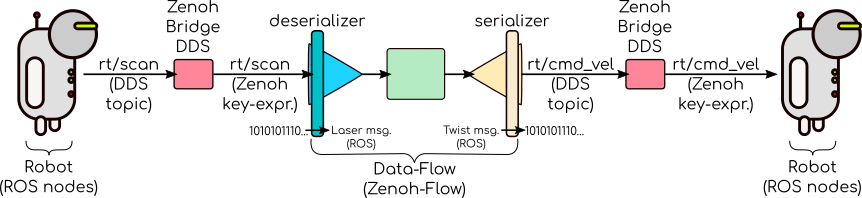
\includegraphics[width=15cm]{figs/zenoh_dds_topology}
  \end{center}
  \caption{Topología software con ROS (DDS) y Zenoh-Flow (Zenoh).}
  \label{fig:zenoh_dds_topology}
\end{figure}\

Además, como podemos ver en la Figura \ref{fig:zenoh_dds_topology}, para que las
\textit{key-expressions} sean traducidas a topics de ROS, deben incluir al
principio de las mismas la partícula \verb|/rt/| en el campo
\textit{key-expression} del archivo de definición de flujo de datos, como el
mostrado en el anterior Código \ref{cod:data_flow_example}.












\chapter{Conclusiones}
\label{cap:capitulo5}

\begin{flushright}
\begin{minipage}[]{10cm}
\emph{Quizás algún fragmento de libro inspirador...}\\
\end{minipage}\\

Autor, \textit{Título}\\
\end{flushright}

\vspace{1cm}

Escribe aquí un párrafo explicando brevemente lo que vas a contar en este capítulo, que básicamente será una recapitulación de los problemas que has abordado, las soluciones que has prouesto, así como los experimentos llevados a cabo para validarlos. Y con esto, cierras la memoria.

\section{Conclusiones}

Enumera los objetivos y cómo los has cumplido.\\

Enumera también los requisitos implícitos en la consecución de esos objetivos, y cómo se han satisfecho.\\

No olvides dedicar un par de párrafos para hacer un balance global de qué has conseguido, y por qué es un avance respecto a lo que tenías inicialmente. Haz mención expresa de alguna limitación o peculiaridad de tu sistema y por qué es así. Y también, qué has aprendido desarrollando este trabajo.\\

Por último, añade otro par de párrafos de líneas futuras; esto es, cómo se puede continuar tu trabajo para abarcar una solución más amplia, o qué otras ramas de la investigación podrían seguirse partiendo de este trabajo, o cómo se podría mejorar para conseguir una aplicación real de este desarrollo (si es que no se ha llegado a conseguir).

\section{Corrector ortográfico}

Una vez tengas todo, no olvides pasar el corrector ortográfico de \LaTeX a todos tus ficheros \textit{.tex}. En \texttt{Windows}, el propio editor \texttt{TeXworks} incluye el corrector. En \texttt{Linux}, usa \texttt{aspell} ejecutando el siguiente comando en tu terminal:

\begin{verbatim}
aspell --lang=es --mode=tex check capitulo1.tex
\end{verbatim}


\chapter{Conclusiones}
\label{cap:capitulo5}

\begin{flushright}
\begin{minipage}[]{10cm}
\emph{Quizás algún fragmento de libro inspirador...}\\
\end{minipage}\\

Autor, \textit{Título}\\
\end{flushright}

\vspace{1cm}

Escribe aquí un párrafo explicando brevemente lo que vas a contar en este capítulo, que básicamente será una recapitulación de los problemas que has abordado, las soluciones que has prouesto, así como los experimentos llevados a cabo para validarlos. Y con esto, cierras la memoria.

\section{Conclusiones}

Enumera los objetivos y cómo los has cumplido.\\

Enumera también los requisitos implícitos en la consecución de esos objetivos, y cómo se han satisfecho.\\

No olvides dedicar un par de párrafos para hacer un balance global de qué has conseguido, y por qué es un avance respecto a lo que tenías inicialmente. Haz mención expresa de alguna limitación o peculiaridad de tu sistema y por qué es así. Y también, qué has aprendido desarrollando este trabajo.\\

Por último, añade otro par de párrafos de líneas futuras; esto es, cómo se puede continuar tu trabajo para abarcar una solución más amplia, o qué otras ramas de la investigación podrían seguirse partiendo de este trabajo, o cómo se podría mejorar para conseguir una aplicación real de este desarrollo (si es que no se ha llegado a conseguir).

\section{Corrector ortográfico}

Una vez tengas todo, no olvides pasar el corrector ortográfico de \LaTeX a todos tus ficheros \textit{.tex}. En \texttt{Windows}, el propio editor \texttt{TeXworks} incluye el corrector. En \texttt{Linux}, usa \texttt{aspell} ejecutando el siguiente comando en tu terminal:

\begin{verbatim}
aspell --lang=es --mode=tex check capitulo1.tex
\end{verbatim}


\clearpage
\thispagestyle{empty}

\printindex \nocite{*}
\appendix
\bibliographystyle{apalike} \bibliography{bibliografia}

\end{document}
